% Initial version by Darian Muresan, Ph.D.
% Edit and adjust as needed.

\documentclass[12pt]{cornell}

% add index support
\makeindex

% graphing programs
\usepackage{color}
\usepackage{psfrag}
\usepackage{verbatim}
\usepackage{fancyhdr}
\usepackage{minted}
%\usepackage{titlesec}
\usepackage{fancyvrb} 
% hyperlink programs
\usepackage[luatex, 
breaklinks=true, 
colorlinks=true,
citecolor=blue,
linkcolor=blue,
menucolor=black,
pagecolor=black,
urlcolor=blue
]{hyperref} % links in pdf
%\usepackage[colorlinks]{hyperref} % links in dvi
\usepackage{listings}
\usepackage{amsfonts} 
\usepackage{amssymb} 
%\usepackage{tabto}

\usepackage{tabularx,colortbl}
\usepackage[chapter]{algorithm} 
\usepackage{algorithmic} 
\usepackage{blindtext}
\usepackage{imakeidx}

% for electronics:
\usepackage[american]{circuitikz}

\definecolor{DarkGreen}{rgb}{0,0.6,0}
\definecolor{mygreen}{rgb}{0,0.6,0}
\definecolor{mygray}{rgb}{0.5,0.5,0.5}
\definecolor{mymauve}{rgb}{0.58,0,0.82}

\usepackage{tocloft}
\usepackage{amsmath}
\usepackage{tcolorbox}
\usepackage{enumitem}
\usepackage{longtable}
%\usepackage{textcomp}
\usepackage{txfonts}

%part for \part titles
%chap for \chapter titles
%sec for \section titles
%subsec for \subsection titles
%subsubsec for \subsubsection titles
%para for \paragraph titles
%subpara for \subparagraph titles
%fig for figure \caption titles
%subfig for subfigure \caption titles
%tab for table \caption titles
%subtab for subtable \caption titles

% update chapter number spacing
\setlength{\cftchapnumwidth}{2em}
\setlength{\cftsecnumwidth}{2.5em}
\setlength{\cftsubsecnumwidth}{3.5em}
\setlength{\cftsubsubsecnumwidth}{4.5em}

\addtolength{\cftsecindent}{0.5em}
\addtolength{\cftsubsecindent}{0.5em}
\addtolength{\cftsubsubsecindent}{0.5em}

%\titlespacing*{\chapter}{0pt}{-50pt}{20pt}
%\titleformat{\chapter}[display]{\normalfont\huge\bfseries}{\chaptertitlename\ 
%\thechapter}{20pt}{\Huge}
%\pagestyle{fancy}
%\pagestyle{cornell}
%
%\rhead{F054-021-0172}
%\chead{Nonlinear Enhancement of Visual Target Detection (AF05-T021)}
%\lhead{GSTI}
%\lfoot{\scriptsize Use or disclosure of data on this page is subject
%to the restriction on the title page of this proposal.}
%\cfoot{}
%\rfoot{\thepage}

\newfont{\Bp}{msbm10}
\newfont{\BpBig}{msbm10 scaled\magstep2}
\newfont{\Sc}{eusm10}
\newfont{\ScBig}{eusm10 scaled\magstep3}
\newfont{\Fr}{eufm10}
\newfont{\FrBig}{eufm10 scaled\magstep1}

% some commands:
\newcommand{\dxi}{{\tt m\_xDeltaInput}}
\newcommand{\dyi}{{\tt m\_yDeltaInput}}
\newcommand{\dci}{{\tt m\_cDeltaInput}}
\newcommand{\dxo}{{\tt m\_xDeltaOutput}}
\newcommand{\dyo}{{\tt m\_yDeltaOutput}}
\newcommand{\dco}{{\tt m\_cDeltaOutput}}
\newcommand{\ttf}[1]{{\tt #1}}
\newcommand{\tbl}[2]{{\begin{tabular}{c} #1 \\ #2 \end{tabular}}}

\newcommand{\urltwo}[2]{\mbox{\href{#1}{\tt #2}}}
\newcommand{\qnorm}[1]{\|#1\|_{\bQ}}
\newcommand{\qdot}[2]{\lrb #1, #2 \rrb_{\bQ}}
\newcommand{\kdot}[2]{\lrb #1, #2 \rrb_{\bf k}}
\newcommand{\tdot}[2]{\lrb #1, #2 \rrb}
\newcommand{\mydiff}[2]{\lrb #1 - #2 \rrb}
\newcommand{\lena}{\textit{lena}}
\newcommand{\barb}{\textit{barbara}}
\newcommand{\boat}{\textit{boat}}
\newcommand{\leaves}{\textit{leaves}}
\newcommand{\rings}{\textit{rings}}
\newcommand{\treg}{\textit{train region}}
\newcommand{\dreg}{\textit{denoise region}}
\newcommand{\oreg}{\textit{overlap region}}
\newcommand{\sil}{\sigma_l^2}
\newcommand{\sn}{\sigma^2}
\newcommand{\bn}{{\mbox{\bf \FrBig N}}}
\newcommand{\n}{\mbox{\Fr N}}
%\newcommand{\bn}{\bf N}
%\newcommand{\n}{N}
\newcommand{\bY}{\textbf{Y}}
\newcommand{\bX}{\textbf{X}}
\newcommand{\bb}{\textbf{b}}
\newcommand{\bu}{\textbf{u}}
\newcommand{\bv}{\textbf{v}}
\newcommand{\by}{\textbf{y}}
\newcommand{\bx}{\textbf{x}}
\newcommand{\be}{\textbf{e}}
\newcommand{\bz}{\textbf{z}}
\newcommand{\bs}{\textbf{s}}
\newcommand{\bw}{\textbf{w}}
\newcommand{\bQ}{\textbf{Q}}
\newcommand{\bphi}{\textbf{$\phi$}}
\newcommand{\lsb}{\left[}
\newcommand{\rsb}{\right]}
\newcommand{\lrb}{\left(}
\newcommand{\rrb}{\right)}
\newcommand{\lcb}{\left\{}
\newcommand{\rcb}{\right\}}
\newcommand{\R}{\mbox{\BpBig R}}
\newcommand{\F}{{\cal F}}
\newcommand{\Fk}{\mbox{\Sc F}}
\newcommand{\bQF}{\textbf{Q}_{\mbox{\Sc F}}}
\newcommand{\N}{{\cal N}}
\newcommand{\xlz}{X_l(z)}
\newcommand{\xhz}{X_h(z)}
\newcommand{\xz}{X(z)}
\newcommand{\pr}{ perfect reconstruction }
\newcommand{\smb}{Smith-Barnwell }
\newcommand{\xw}{X(e^{j\omega})}
\newcommand{\xmw}{X(-e^{j\omega})}
\newcommand{\dw}{D(e^{j\omega})}
\newcommand{\dmw}{D(-e^{j\omega})}
\newcommand{\ew}{E(e^{j\omega})}
\newcommand{\emw}{E(-e^{j\omega})}
\newcommand{\fw}{F_0(e^{j\omega})}
\newcommand{\fmw}{F_0(-e^{j\omega})}
\newcommand{\hoz}{H_1(z)}
\newcommand{\hzz}{H_0(z)}
\newcommand{\goz}{G_1(z)}
\newcommand{\gzz}{G_0(z)}
\newcommand{\hzw}{H_{0}(e^{j\omega})}
\newcommand{\hzmw}{H_{0}(-e^{j\omega})}
\newcommand{\hzcw}{H_{0}(e^{-j\omega})}
\newcommand{\how}{H_1(e^{j\omega})}
\newcommand{\homw}{H_1(-e^{j\omega})}
\newcommand{\gzw}{G_0(e^{j\omega})}
\newcommand{\gzmw}{G_0(-e^{j\omega})}
\newcommand{\gow}{G_1(e^{j\omega})}
\newcommand{\gomw}{G_1(-e^{j\omega})}
\newcommand{\wl}{e^{-jwL}}
\newcommand{\aqua}{\textit{AQua with OR }}
\newtheorem{theorem}{Theorem}
\newtheorem{lemma}{Lemma}
\newtheorem{corollary}{Corollary}
\newtheorem{claim}{Claim}
\newtheorem{definition}{Definition}
\newenvironment{proof}{\noindent{\em Proof.}}{\ \hfill Q.E.D.}
%\newtheorem{moduleCount}{L}
\newcommand*{\labelfile}[1]{%
  \label{file:#1}%
}

\lstset{ %
  backgroundcolor=\color{white},   % choose the background color; you must add \usepackage{color} or \usepackage{xcolor}
  basicstyle=\footnotesize,        % the size of the fonts that are used for the code
  breakatwhitespace=false,         % sets if automatic breaks should only happen at whitespace
  breaklines=true,                 % sets automatic line breaking
  captionpos=b,                    % sets the caption-position to bottom
  commentstyle=\color{DarkGreen},    % comment style
  deletekeywords={...},            % if you want to delete keywords from the given language
  escapeinside={\%*}{*)},          % if you want to add LaTeX within your code
  extendedchars=true,              % lets you use non-ASCII characters; for 8-bits encodings only, does not work with UTF-8
  %frame=single,                   % adds a frame around the code
  keepspaces=true,                 % keeps spaces in text, useful for keeping indentation of code (possibly needs columns=flexible)
  keywordstyle=\color{blue},       % keyword style
  language=C++,                    % the language of the code
  morekeywords={*,...},            % if you want to add more keywords to the set
  numbers=left,                    % where to put the line-numbers; possible values are (none, left, right)
  numbersep=5pt,                   % how far the line-numbers are from the code
  numberstyle=\tiny\color{mygray}, % the style that is used for the line-numbers
  rulecolor=\color{black},         % if not set, the frame-color may be changed on line-breaks within not-black text (e.g. comments (green here))
  showspaces=false,                % show spaces everywhere adding particular underscores; it overrides 'showstringspaces'
  showstringspaces=false,          % underline spaces within strings only
  showtabs=false,                  % show tabs within strings adding particular underscores
  stepnumber=1,                    % the step between two line-numbers. If it's 1, each line will be numbered
  stringstyle=\color{mymauve}     % string literal style
  %tabsize=2,                      % sets default tabsize to 2 spaces
  %caption=\lstname                % show the filename of files included with \lstinputlisting; also try caption instead of title
}

% Uncomment draftcopy to get the word DRAFT boldly across the first page
%   By the way, xdvi won't show it but it will come out when you print
%\usepackage[light,all]{draftcopy}		% DRAFT on first page
%\draftcopySetGrey{.97}
%\draftcopyName{Confidential}{150}
%\draftcopFirstPage{1}

% Uncomment drafthead to get the date and DRAFT in the header of pages
% that are normallly numbered on the top, pages 2-n of each chapter for example
% This doesn't work with centered page numbers: \pagestyle{cornellc}
%\usepackage{drafthead}

% Including selective chapters:
% use this to selectively process chapters, etc.  Put a % in front of
% the sections that you don't want done this time.  Includes are
% used instead of \input so that LaTeX will keep track of chapters and
% pages without processing everything.  Don't let any spaces creep in
% around the words or it will not work!


\includeonly{
prologue,
manIntroduction,
manProjectDescription,
manResources,
manRadarTheory,
manPartSelection,
manPCB,
manDigitalProcessing,
manNetworking,
manResults,
manIssues
}

\makeindex

\begin{document}

\pagenumbering{roman}
\singlespacing
% File: prologue.tex
% Thesis prologue:  Title page, acknowledgements, table of contents,
% list of figures, and list of tables.
%
% this file is to be \include'd after the \begin{document}

% Cornell-style title page
\begin{titlepage}
        \title{Mithril - FMCW Radar}
        \author{Tomas Esson, Ajay Thakkar, Juan Jimenez \\ tesson@stevens.edu, athakka5@stevens.edu, jjimene6@stevens.edu }
        \conferraldate{}{\today} \maketitle
\end{titlepage}

% Copyright page
%\begin{copyrightpage}
\makecopyright
%\end{copyrightpage}

% Abstract: the abstract body is pulled from the file abstract.tex;
%  the title is pulled from the \title command in the titlepage section

% Biographical information pulled from file bio.tex
%\begin{biosketch} \input bio \end{biosketch}

% Dedication (optional):  pulls information from file dedication.tex
%\begin{dedication} 
%\input dedicate 
%\end{dedication}

% Acknowledgements:  pulls information from file acknow
%\begin{acknowledgements} \input acknow \end{acknowledgements}

% Table of contents
\contentspage

% If you have no tables or figures put a % in front of the list page line
% List of tables
\tablelistpage

% List of figures
\figurelistpage



\setcounter{page}{1}        % set page counter
\pagenumbering{arabic}      % set page number style
\pagestyle{fancy}         % top right page numbers
%\pagestyle{cornell}
%\pagestyle{cornellc}       % centered page numbers, disables drafthead

\renewcommand{\chaptermark}[1]{\markboth{#1}{}}
\renewcommand{\sectionmark}[1]{\markright{#1}{}}

\fancyhead{} % clear all fields

\lhead{Chapter \thechapter}
%\lhead{\thechapter}
\chead{\leftmark}
\rhead{\thepage}


\lfoot{Chapter \thechapter}
\cfoot{\copyright Stevens -- \today \mbox{} -- FPGA Radio Receiver/Transmitter}
\rfoot{\thepage}

\renewcommand{\headrulewidth}{0.4pt}
\renewcommand{\footrulewidth}{0.4pt}

%\rhead{F054-021-0172}
%\chead{Nonlinear Enhancement of Visual Target Detection (AF05-T021)}
%\lhead{GSTI}
%\lfoot{\scriptsize Use or disclosure of data on this page is subject
%to the restriction on the title page of this proposal.}
%\cfoot{}
%\rfoot{\thepage}


\singlespacing
\chapter{Introduction 
\index{Chapter!Introduction}
\index{Introduction}
\label{Introduction}}

The following includes small biographies on all the authors as well as their research interests and projects.

\section*{Authors' Biographies}
\subsection*{Ajay Thakkar}
\textbf{Ajay Thakkar} Ajay Thakkar is a junior majoring in Computer Engineering. He is interested in signal processing and lower level coding. Below you can find his GitHub: \url{https://github.com/athakkar2}.

\subsection*{Tomas Esson}
\textbf{Tomas Esson} is an aspiring Computer Engineering at Stevens Institute of technology. He is an avid surfer and enjoys elegant math proofs. Currently pursuing interests in computer chip design, digital systems implementation, mathematical optimization of computer chips, and electrical engineering. 

\subsection*{Juan Jimenez}
\textbf{Juan Jimenez} is a Junior Computer Engineering student at the Stevens Institute of technology. Interested in the intersection between Artificial Intelligence, embedded electronics, and software engineering. To see more projects visit the following GitHub link: \url{https://github.com/jjimene1}  
\chapter{Project Description 
\index{Chapter!Project Description}
\index{Project Description}
\label{Project Description}}
\begin{figure}[H]
  \centering
  \begin{tikzpicture}[node distance = 2cm, auto]
      % Define block styles
      \tikzstyle{block} = [rectangle, draw, fill=blue!20, 
          text width=5em, text centered, rounded corners, minimum height=4em]
      \tikzstyle{line} = [draw, ->]
  
      % Place nodes
      \node [block] (mithril) {Mithril};
      \node [block, below of=mithril, node distance=4cm] (radar) {FMCW Radar};
      \node [block, left of=radar, node distance=4cm] (processing) {Digital Processing};
      \node [block, right of=radar, node distance=4cm] (networking) {Distributed Networking};
      \node [block, below of=processing, node distance=2cm] (STM) {STM MC and Python};
      \node [block, below of=radar, node distance=2cm] (ORCad) {Cadence ORCad};
      \node [block, below of=networking, node distance=2cm] (pi) {Raspberry Pi and MQTT};
      % Draw edges
      \path [line] (mithril) -- (radar);
      \path [line] (mithril) -- (processing);
      \path [line] (mithril) -- (networking);
      \path [line] (radar) -- (ORCad);
      \path [line] (processing) -- (STM);
      \path [line] (networking) -- (pi);
  \end{tikzpicture}
  \caption{Flowchart of the Mithril system}
  \label{fig:mithril_flowchart}
  \end{figure}
Mithril is a nodal FMCW radar system that incorporates traditional FMCW radar,
digital processing, edge computing, and distributed networking. The initial idea of this 

As can be seen in Figure \ref{fig:mithril_flowchart},
the radar was designed as a standalone PCB in ORCad, digital processing was handled by
STM microcontrollers, and distributed networking is done via Raspberry Pi's and the MQTT protocol.
All of these components were designed, engineered, and interfaced from scratch with a limited budget
of 2000 dollars.

\section{}
The heart of the project is a standalone PCB capable of FMCW radar.
\chapter{Resources
\index{Chapter!Resources}
\index{Resources}
\label{Resources}}
\chapter{Radar Theory
\index{Chapter!Radar Theory}
\index{Radar Theory}
\label{Radar Theory}}

\section{Getting Started}



include the benefits of using higher frequency signals

heterodyning
\chapter{Part Selection
\index{Chapter!Part Selection}
\index{Part Selection}
\label{Part Selection}}

\begin{figure}[H]
  \centering
  \scalebox{.8}{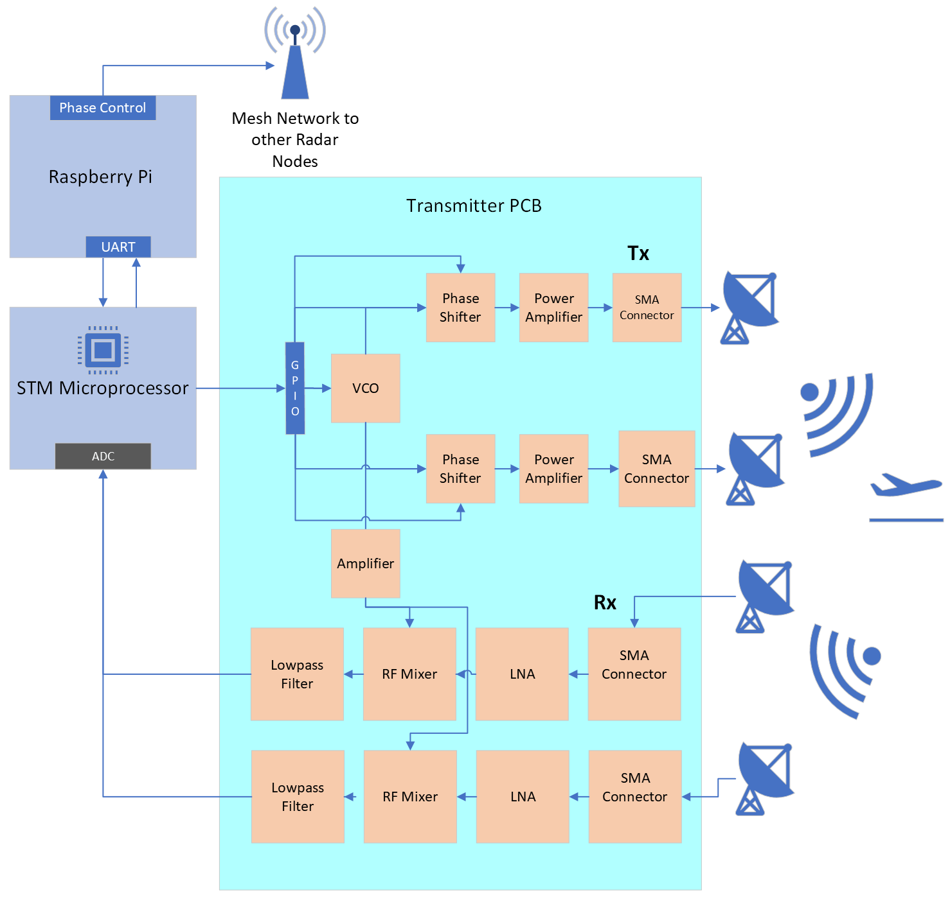
\includegraphics{Diagrams/overview.png}}
\caption{Architecture Overview}
\label{img:projoverview}
\end{figure}

In this chapter, we will go through the architecture of the PCB and show what parts we picked and what purposes they serve.
Figure \ref{img:projoverview} shows the overall architecture of the project.

\section{Voltage Controlled Oscillator (VCO)}
The first step in creating a radar is signal synthesis. You essentially need to create an alternating current signal that can
go through your antenna and radiate out into the air. To reiterate from Chapter \ref{Radar Theory}, higher frequency signals are
important for a better radar resolution, and so it is desired to have a signal that is high in frequency. Naively, at the
beginning of this project we thought we could use a 16 bit DAC to synthesize our signal but after finding out its max clock rate 
was 1 MHz, we realized a DAC was not fit for this. All we needed was something that could create a simple sinusoid at a very
high frequency.

Voltage Controlled Oscillators (VCO) do just this. They take in a "tuning voltage" which corresponds to a certain frequency
of sinusoid which it will output. The circuitry for this is beyond me, but for a good overall guide on VCOs you can check out
DigiKey's article \href{https://www.digikey.com/en/articles/the-basics-of-voltage-controlled-oscillators-vcos}{here}.

Now that we knew how to synthesize our signal, it was important to find a good VCO that had a high output bandwidth. Whatever
bandwidth the VCO has will impact what parts we can get in the other stages of the RF chain since these must be within the VCOs
operating regions. 

\begin{figure}[H]
    \centering
    \scalebox{.7}{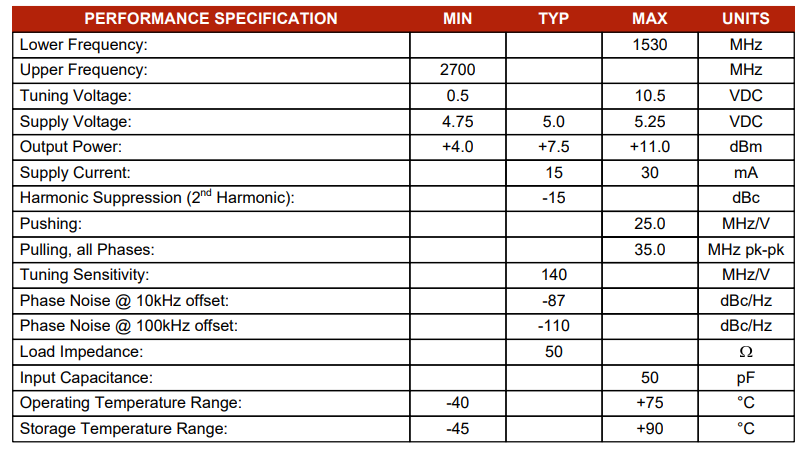
\includegraphics{DatasheetImages/vcotable.png}}
    \caption{VCO Datasheet Table}
    \label{img:vcotable}
\end{figure}
\begin{figure}[H]
    \centering
    \scalebox{.7}{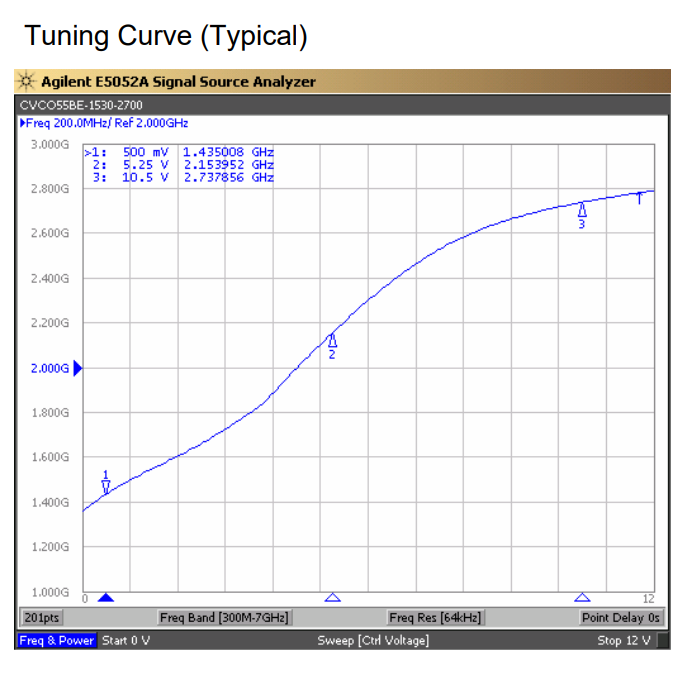
\includegraphics{DatasheetImages/vcotuningtable.png}}
    \caption{Tuning Voltage Graph}
    \label{img:tuninggraph}
\end{figure}

We chose a VCO from Crystek which can be found on Digikey \href{https://www.digikey.com/en/products/detail/crystek-corporation/CVCO55BE-1530-2700/1644030}{here}.
Looking at the specifications table in Figure \ref{img:vcotable}, some good things to look for are first and foremost the frequency
range of the part. It goes from about 1.5-2.7 GHz, which is a pretty wide range and would support a lot of other parts as it also
covers the Wi-Fi band. The second thing to look for is output power. The output power can be a constraint for other parts, since they
might have a absolute limit on their input power, and it is useful to know the output power for finding out how strong your signal will be
once it propogates out of your antenna. Here we can see the output power is around 7.5 dBm, and this will be split four ways. 
Decibels are a logarithmic scale, so we cannot just divide by four but instead use a decibel calculator like \href{https://noisetools.net/decibelcalculator}{this one}.

Now, another key metric is the tuning voltage. Luckily, this Crystek provides a tuning voltage graph found in Figure \ref{img:tuninggraph}
that shows us how the output frequency changes with changes in the tuning voltage. One observation is that it is not linear, meaning
our ramp voltage will not result in a true linear ramp in frequency. Another observation is that our chosen frequency of 1.8 GHz is
around 3.5 volts following the graph. Our STM board that will generate the ramp voltage can by default only go to 3.3 volts, but we
found a workaround to go to 5 volts which allowed us to stick with our decided center frequency.

\section{Power Divider}
As mentioned before, we want to divide the VCO's signal four ways because want it to go to two phase shifters, and two mixers.
At first we thought it was as simple as having one wire split into four, but as we will go over in Chapter \ref{PCB}, impedence
matching is very important in RF circuits. To put it simply, impedance matching ensures that no power is reflected, and this is
important because reflected power means distortions in the signal and power loss. That means we needed a power splitter meant for
splitting an RF signal without causing reflected power. There is not much of note with the part we used which can be found 
\href{https://www.mouser.com/ProductDetail/Mini-Circuits/WP4P1%2B?qs=Imq1NPwxi77kWybHhilv%2Fg%3D%3D}{here}. The main thing is that
it contains the frequency of 1.8 GHz we want to use.

\section{Phase Shifter}
Two of the power dividers split paths will go into phase shifters. The phase shifters are used to make our phased array
of antennas as explained in Chapter \ref{Radar Theory}. They are able to change the phase (add time delay), to the signal 
so that when they propogate through the air they can construct and destruct. The phase shifters we chose can be found
\href{https://www.digikey.com/en/products/detail/psemi/PE44820B-X/5822957}{here}. These are digital phase shifters that have 256
different phases it can apply to the signal. They have a parallel or serial interface we can use to transmit 8 bit words That
will alter the phase of our signal. The interface and its timing diagrams will be explained more in detail in Chapter \ref{Digital Processing}.
All we need to know is that the bandwidth that the chip supports contains 1.8 GHz.

\section{Power Amplifier}
\begin{figure}[H]
  \centering
  \scalebox{.6}{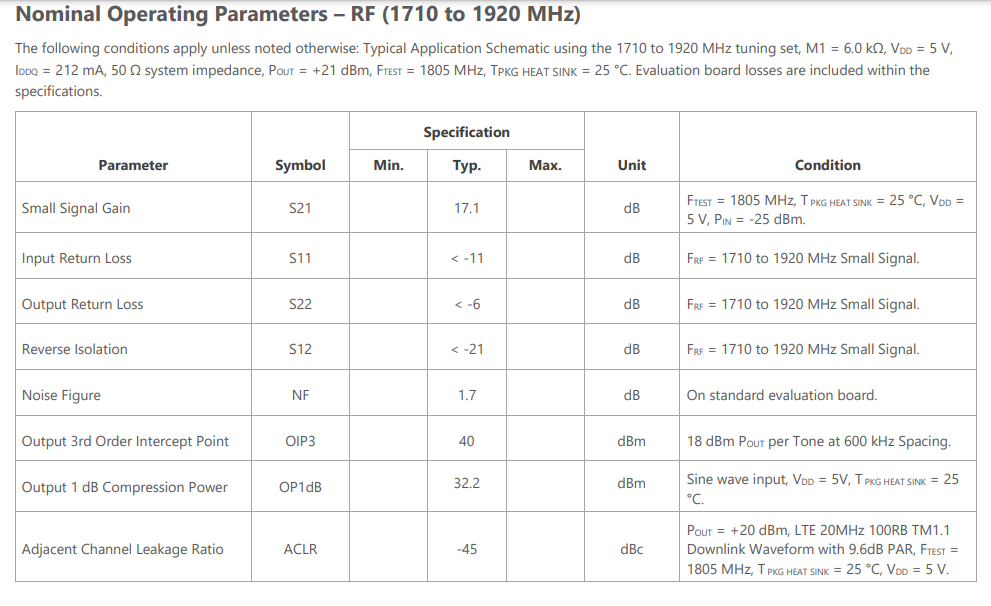
\includegraphics{DatasheetImages/poweramptable.png}}
  \caption{Power Amplifier Table}
  \label{img:poweramptable}
\end{figure}
At this point after the VCO and phase shifter, we want the RF signal to propogate through the air. However, according to the
radar range equation the power of the signal when attenuating through the air attenuates at a power of four which is a lot.
Therefore, we need to make sure our signal is powerful enough to go pretty far. So, we use an RF power amplifier to amplify the
signal. We chose a part from GuerillaRF which can be found \href{https://www.mouser.com/ProductDetail/Guerrilla-RF/GRF5112?qs=ulEaXIWI0c%252Bti188Qa1Now%3D%3D}{here}.
Looking at the table in Figure \ref{img:poweramptable}, we can see some key metrics when looking at power amplifiers. First,
of course we want to make sure it has a bandwidth that supports our chosen frequency of 1.8 GHz. Second, we want to look at the
small-signal gain and Output 1 dB Compression Point or OP1dB. The small-signal gain is the ideal gain that can be reached with a 
low power signal, and is listed as 17.1 dB. The OP1dB is a metric we did not know about and were thankful to find it. With most amplifiers,
gain operates linearly meaning whatever power your input signal is you just add the gain of the amplifier and this will be the resulting power of the signal.
However, at a certain point the amplifier saturates and does not operate linearly anymore, and will essentially cap-off its gain at
the OP1dB limit. For example, with the OP1dB being 32.2 dB, if I input a signal that was 30 dB I would expect a resulting signal of
47.1 dB but this would not be the case. The amplifier ceases to operate linearly after the 32.2 dB mark, and will both distort the signal
and output something weaker than expected. A lot of amplifiers will boast a high gain but have a low OP1dB, so this is definitely something to check for.

\section{Low Noise Amplifier}
\begin{figure}[H]
  \centering
  \scalebox{.7}{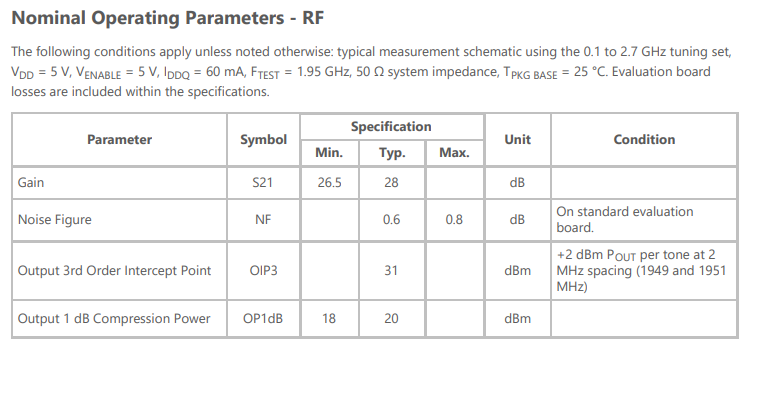
\includegraphics{DatasheetImages/lnatable.png}}
  \caption{Low-Noise Amplifier Table}
  \label{img:lnatable}
\end{figure}

This is the first part that will be placed in the receiver RF chain. According to the Friis equation in Chapter \ref{Radar Theory},
the first stage in the receiver RF chain matters a lot for the noise figure of your system. Therefore, we wanted to find a part
with a low noise figure and high gain, as this will impact our SNR the most. Low noise amplifiers are made for this exact purpose,
where they amplify a small signal with very low noise. The part we chose was \href{https://www.mouser.com/ProductDetail/Guerrilla-RF/GRF2133W?qs=ulEaXIWI0c%2FXgAPwqRmr2A%3D%3D}{this},
which is made by GuerillaRF. By examining the table in Figure \ref{img:lnatable}, we can see that it has a gain of 28 dB,
and a noise figure of .6 dB. We also can look at the OP1dB which has a figure of 20 dB. Since the LNA will be amplifying a signal
straight from an antenna, the signal will be super weak and there is a low likelihood it will reach the OP1dB.

\section{Mixer/LO Amp}
\begin{figure}[H]
  \centering
  \scalebox{.7}{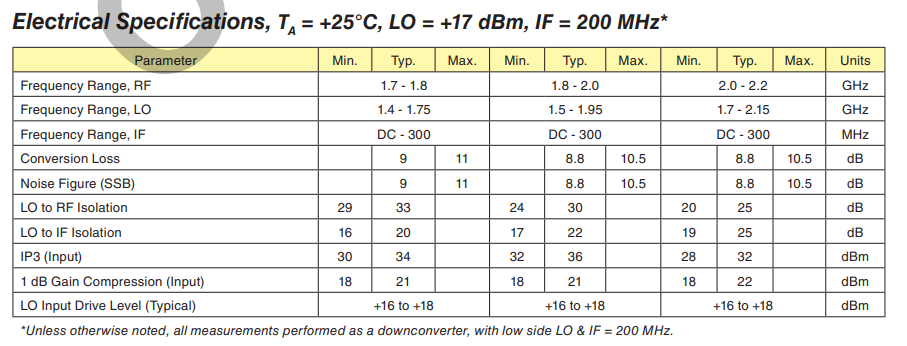
\includegraphics{DatasheetImages/mixertable.png}}
  \caption{Mixer Table}
  \label{img:mixertable}
\end{figure}
\begin{figure}[H]
  \centering
  \scalebox{.7}{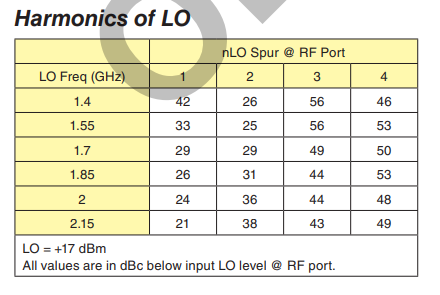
\includegraphics{DatasheetImages/mixerharmonics.png}}
  \caption{Mixer Harmonics Table}
  \label{img:mixerharmonics}
\end{figure}

Now that our received signal is amplified we must down-convert it in order to sample and process it. The process for doing
this is called heterodyning or mixing, and the theory behind this can be found in detail in Chapter \ref{Radar Theory}. 
A mixer has three ports, the local oscillator, RF signal, and output. The local oscillator and RF signal are multiplied
to produce the sum and difference of the LO and RF signals on the output port. We are mainly interested in the difference,
also called the Intermediate Frequency (IF) since it is a low frequency and can be sampled easily.
In our case, we take a copy of the VCO as the local oscillator and then mix this with the amplified return signal 
to produce our intermediate frequency. To achieve this, we used a discontinued mixer from Analog Devices which
can be found \href{https://www.arrow.com/en/products/hmc400ms8etr/analog-devices}{here}. 
Looking at the mixer's specifications table in Figure \ref{img:mixertable}, we can 
see some new properties. The conversion loss is the output IF power delivered minus the available RF input signal power. The
LO to RF Isolation is how much of the local oscillator signal leaks into the RF port, and the LO to IF Isolation is how much
the local oscillator signal leaks into the output port. This is a passive component, meaning it does not require power and
solely operates off the power of the LO and RF signals. Therefore we see in the table that the LO Input must be 16-18 dBm to drive
the mixer. Essentially the local oscillator powers the mixer, and its harmonics will therefore be prominent in the IF port due to
leakage. We can see in Figure \ref{img:mixerharmonics} that at 1.85 GHz the manufacturer tells us the strength of LO harmonics 
up to the fourth order. At the top it says spur which means spurious (unwanted) outputs due to the nonlinearity of the mixer.
Essentially this table tells us that there will be unwanted spectral components in the output, which is something we did not
pay enough attention to and will discuss in Chapter \ref{Issues}.
\begin{figure}[H]
  \centering
  \scalebox{.7}{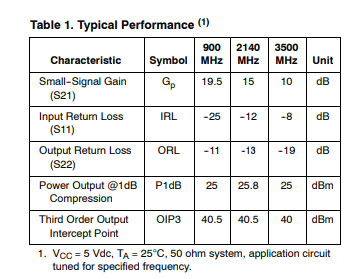
\includegraphics{DatasheetImages/loamptable.png}}
  \caption{LO Amp Table}
  \label{img:loamptable}
\end{figure}

As we said before, the mixer is a passive component which is driven by the LO which needs a power level of 16-18 dBm.
After splitting our VCO's output four ways, we have about a ~2 dBm signal that we must amplify. So, we chose an RF broadband
amplifier from NXP which can be found \href{https://www.digikey.com/en/products/detail/nxp-usa-inc/MMG3014NT1/1971761}{here}. As
we can see in Figure \ref{img:loamptable}, the amp has a gain of around 15 dB for our frequency and an OP1dB of 25.8 dB which is
a lot of headroom.

\section{IF Amplifiers and Filters}
Now, our return signal has been downconverted, but the power of that signal is very weak. As well as this, there are unwanted
spectral components in that signal that are bi-products of the mixer that we need to get rid of. This means we need amplifiers and
filters to make our signal ready to be sampled and processed in the microcontroller. First we used a super simple op-amp
that served as a voltage follower which can be found \href{https://www.digikey.com/en/products/detail/microchip-technology/MCP6001UT-I-OT/562450}{here}.
This was used to create a virtual ground for our biasing. Then we use a dual channel op-amp from TI for our variable gain
amplifier which can be found \href{https://www.mouser.com/ProductDetail/Texas-Instruments/LM2904DR?qs=5BZzbFV4k2vkQqOl3Q8qPg%3D%3D}{here}.

\begin{figure}[H]
  \centering
  \scalebox{.7}{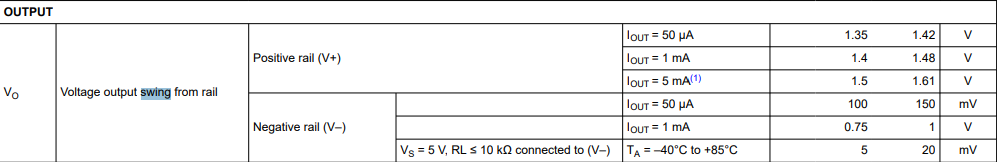
\includegraphics{DatasheetImages/outputswing.png}}
  \caption{Output Swing Characteristics}
  \label{img:outputswing}
\end{figure}

Honestly, when selecting parts we figured all operational amplifiers just acted the same way. However, after printing and manufacturing
we ran into problems which will be discussed in Chapter \ref{Issues} that could have been remedied if we paid more attention to
the Op-Amps we were using. The main problem is that these operational amplifiers are not "Rail-to-Rail".
While rail-to-rail amplifiers guarantee that they do not saturate until the positive and negative voltages you've supplied it,
other amplifiers have what is called voltage swing. As we can see in Figure \ref{img:outputswing}, the range of voltage
that the operational amplifier can achieve is not its rails, but specifies how much lower than its rail it will be. This is 
something to look out for when selecting an Op-Amp.

\begin{figure}[H]
  \centering
  \scalebox{.7}{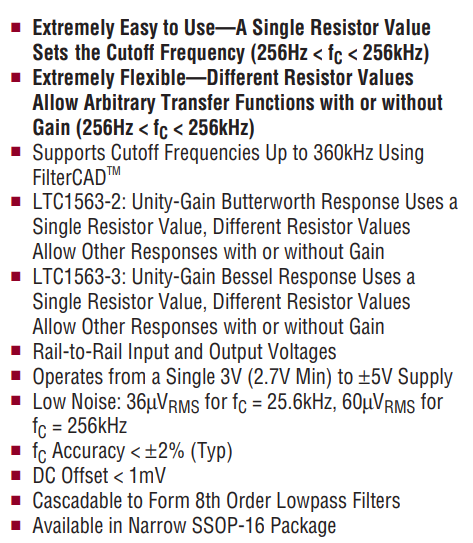
\includegraphics{DatasheetImages/filterspecs.png}}
  \caption{Filter Features}
  \label{img:filterspecs}
\end{figure}

After amplifying the signal, we wanted to filter out unwanted spectral components by using a strong filter. Instead of designing
this ourselves, we decided to use a 4th Order LPF which can be found \href{https://www.digikey.com/en/products/detail/analog-devices-inc/LTC1563-2IGN-PBF/962958}{here}.
By looking at Figure \ref{img:filterspecs}, we can see that this is an integrated circuit with a flexible cutoff frequency.
It also says that it is a rail-to-rail input and output circuit, which is an important feature to note as discussed with the amplifiers.
A fourth order filter just means that this filter has four filters with the same cutoff frequency cascaded upon each other, which
yields a steeper frequency response and attenuates are unwanted signals further.
\chapter{PCB
\index{Chapter!PCB}
\index{PCB}
\label{PCB}}
\chapter{Digital Processing
\index{Chapter!Digital Processing}
\index{Digital Processing}
\label{Digital Processing}}
\chapter{Networking
\index{Chapter!Networking}
\index{Networking}
\label{Networking}}


\chapter{Results
\index{Chapter!Results}
\index{Results}
\label{Results}}
\chapter{Issues
\index{Chapter!Issues}
\index{Issues}
\label{Issues}}

%\bibliography{bibfile}
%\bibliographystyle{unsrt}
%\bibliographystyle{IEEEtran}

%% Initial version by Darian Muresan, Ph.D.
% Edit and adjust as needed.

\documentclass[12pt]{cornell}

% add index support
\makeindex

% graphing programs
\usepackage{color}
\usepackage{psfrag}
\usepackage{verbatim}
\usepackage{fancyhdr}
\usepackage{minted}
%\usepackage{titlesec}
\usepackage{fancyvrb} 
% hyperlink programs
\usepackage[luatex, 
breaklinks=true, 
colorlinks=true,
citecolor=blue,
linkcolor=blue,
menucolor=black,
pagecolor=black,
urlcolor=blue
]{hyperref} % links in pdf
%\usepackage[colorlinks]{hyperref} % links in dvi
\usepackage{listings}
\usepackage{amsfonts} 
\usepackage{amssymb} 
%\usepackage{tabto}

\usepackage{tabularx,colortbl}
\usepackage[chapter]{algorithm} 
\usepackage{algorithmic} 
\usepackage{blindtext}
\usepackage{imakeidx}

% for electronics:
\usepackage[american]{circuitikz}

\definecolor{DarkGreen}{rgb}{0,0.6,0}
\definecolor{mygreen}{rgb}{0,0.6,0}
\definecolor{mygray}{rgb}{0.5,0.5,0.5}
\definecolor{mymauve}{rgb}{0.58,0,0.82}

\usepackage{tocloft}
\usepackage{amsmath}
\usepackage{tcolorbox}
\usepackage{enumitem}
\usepackage{longtable}
%\usepackage{textcomp}
\usepackage{txfonts}

%part for \part titles
%chap for \chapter titles
%sec for \section titles
%subsec for \subsection titles
%subsubsec for \subsubsection titles
%para for \paragraph titles
%subpara for \subparagraph titles
%fig for figure \caption titles
%subfig for subfigure \caption titles
%tab for table \caption titles
%subtab for subtable \caption titles

% update chapter number spacing
\setlength{\cftchapnumwidth}{2em}
\setlength{\cftsecnumwidth}{2.5em}
\setlength{\cftsubsecnumwidth}{3.5em}
\setlength{\cftsubsubsecnumwidth}{4.5em}

\addtolength{\cftsecindent}{0.5em}
\addtolength{\cftsubsecindent}{0.5em}
\addtolength{\cftsubsubsecindent}{0.5em}

%\titlespacing*{\chapter}{0pt}{-50pt}{20pt}
%\titleformat{\chapter}[display]{\normalfont\huge\bfseries}{\chaptertitlename\ 
%\thechapter}{20pt}{\Huge}
%\pagestyle{fancy}
%\pagestyle{cornell}
%
%\rhead{F054-021-0172}
%\chead{Nonlinear Enhancement of Visual Target Detection (AF05-T021)}
%\lhead{GSTI}
%\lfoot{\scriptsize Use or disclosure of data on this page is subject
%to the restriction on the title page of this proposal.}
%\cfoot{}
%\rfoot{\thepage}

\newfont{\Bp}{msbm10}
\newfont{\BpBig}{msbm10 scaled\magstep2}
\newfont{\Sc}{eusm10}
\newfont{\ScBig}{eusm10 scaled\magstep3}
\newfont{\Fr}{eufm10}
\newfont{\FrBig}{eufm10 scaled\magstep1}

% some commands:
\newcommand{\dxi}{{\tt m\_xDeltaInput}}
\newcommand{\dyi}{{\tt m\_yDeltaInput}}
\newcommand{\dci}{{\tt m\_cDeltaInput}}
\newcommand{\dxo}{{\tt m\_xDeltaOutput}}
\newcommand{\dyo}{{\tt m\_yDeltaOutput}}
\newcommand{\dco}{{\tt m\_cDeltaOutput}}
\newcommand{\ttf}[1]{{\tt #1}}
\newcommand{\tbl}[2]{{\begin{tabular}{c} #1 \\ #2 \end{tabular}}}

\newcommand{\urltwo}[2]{\mbox{\href{#1}{\tt #2}}}
\newcommand{\qnorm}[1]{\|#1\|_{\bQ}}
\newcommand{\qdot}[2]{\lrb #1, #2 \rrb_{\bQ}}
\newcommand{\kdot}[2]{\lrb #1, #2 \rrb_{\bf k}}
\newcommand{\tdot}[2]{\lrb #1, #2 \rrb}
\newcommand{\mydiff}[2]{\lrb #1 - #2 \rrb}
\newcommand{\lena}{\textit{lena}}
\newcommand{\barb}{\textit{barbara}}
\newcommand{\boat}{\textit{boat}}
\newcommand{\leaves}{\textit{leaves}}
\newcommand{\rings}{\textit{rings}}
\newcommand{\treg}{\textit{train region}}
\newcommand{\dreg}{\textit{denoise region}}
\newcommand{\oreg}{\textit{overlap region}}
\newcommand{\sil}{\sigma_l^2}
\newcommand{\sn}{\sigma^2}
\newcommand{\bn}{{\mbox{\bf \FrBig N}}}
\newcommand{\n}{\mbox{\Fr N}}
%\newcommand{\bn}{\bf N}
%\newcommand{\n}{N}
\newcommand{\bY}{\textbf{Y}}
\newcommand{\bX}{\textbf{X}}
\newcommand{\bb}{\textbf{b}}
\newcommand{\bu}{\textbf{u}}
\newcommand{\bv}{\textbf{v}}
\newcommand{\by}{\textbf{y}}
\newcommand{\bx}{\textbf{x}}
\newcommand{\be}{\textbf{e}}
\newcommand{\bz}{\textbf{z}}
\newcommand{\bs}{\textbf{s}}
\newcommand{\bw}{\textbf{w}}
\newcommand{\bQ}{\textbf{Q}}
\newcommand{\bphi}{\textbf{$\phi$}}
\newcommand{\lsb}{\left[}
\newcommand{\rsb}{\right]}
\newcommand{\lrb}{\left(}
\newcommand{\rrb}{\right)}
\newcommand{\lcb}{\left\{}
\newcommand{\rcb}{\right\}}
\newcommand{\R}{\mbox{\BpBig R}}
\newcommand{\F}{{\cal F}}
\newcommand{\Fk}{\mbox{\Sc F}}
\newcommand{\bQF}{\textbf{Q}_{\mbox{\Sc F}}}
\newcommand{\N}{{\cal N}}
\newcommand{\xlz}{X_l(z)}
\newcommand{\xhz}{X_h(z)}
\newcommand{\xz}{X(z)}
\newcommand{\pr}{ perfect reconstruction }
\newcommand{\smb}{Smith-Barnwell }
\newcommand{\xw}{X(e^{j\omega})}
\newcommand{\xmw}{X(-e^{j\omega})}
\newcommand{\dw}{D(e^{j\omega})}
\newcommand{\dmw}{D(-e^{j\omega})}
\newcommand{\ew}{E(e^{j\omega})}
\newcommand{\emw}{E(-e^{j\omega})}
\newcommand{\fw}{F_0(e^{j\omega})}
\newcommand{\fmw}{F_0(-e^{j\omega})}
\newcommand{\hoz}{H_1(z)}
\newcommand{\hzz}{H_0(z)}
\newcommand{\goz}{G_1(z)}
\newcommand{\gzz}{G_0(z)}
\newcommand{\hzw}{H_{0}(e^{j\omega})}
\newcommand{\hzmw}{H_{0}(-e^{j\omega})}
\newcommand{\hzcw}{H_{0}(e^{-j\omega})}
\newcommand{\how}{H_1(e^{j\omega})}
\newcommand{\homw}{H_1(-e^{j\omega})}
\newcommand{\gzw}{G_0(e^{j\omega})}
\newcommand{\gzmw}{G_0(-e^{j\omega})}
\newcommand{\gow}{G_1(e^{j\omega})}
\newcommand{\gomw}{G_1(-e^{j\omega})}
\newcommand{\wl}{e^{-jwL}}
\newcommand{\aqua}{\textit{AQua with OR }}
\newtheorem{theorem}{Theorem}
\newtheorem{lemma}{Lemma}
\newtheorem{corollary}{Corollary}
\newtheorem{claim}{Claim}
\newtheorem{definition}{Definition}
\newenvironment{proof}{\noindent{\em Proof.}}{\ \hfill Q.E.D.}
%\newtheorem{moduleCount}{L}
\newcommand*{\labelfile}[1]{%
  \label{file:#1}%
}

\lstset{ %
  backgroundcolor=\color{white},   % choose the background color; you must add \usepackage{color} or \usepackage{xcolor}
  basicstyle=\footnotesize,        % the size of the fonts that are used for the code
  breakatwhitespace=false,         % sets if automatic breaks should only happen at whitespace
  breaklines=true,                 % sets automatic line breaking
  captionpos=b,                    % sets the caption-position to bottom
  commentstyle=\color{DarkGreen},    % comment style
  deletekeywords={...},            % if you want to delete keywords from the given language
  escapeinside={\%*}{*)},          % if you want to add LaTeX within your code
  extendedchars=true,              % lets you use non-ASCII characters; for 8-bits encodings only, does not work with UTF-8
  %frame=single,                   % adds a frame around the code
  keepspaces=true,                 % keeps spaces in text, useful for keeping indentation of code (possibly needs columns=flexible)
  keywordstyle=\color{blue},       % keyword style
  language=C++,                    % the language of the code
  morekeywords={*,...},            % if you want to add more keywords to the set
  numbers=left,                    % where to put the line-numbers; possible values are (none, left, right)
  numbersep=5pt,                   % how far the line-numbers are from the code
  numberstyle=\tiny\color{mygray}, % the style that is used for the line-numbers
  rulecolor=\color{black},         % if not set, the frame-color may be changed on line-breaks within not-black text (e.g. comments (green here))
  showspaces=false,                % show spaces everywhere adding particular underscores; it overrides 'showstringspaces'
  showstringspaces=false,          % underline spaces within strings only
  showtabs=false,                  % show tabs within strings adding particular underscores
  stepnumber=1,                    % the step between two line-numbers. If it's 1, each line will be numbered
  stringstyle=\color{mymauve}     % string literal style
  %tabsize=2,                      % sets default tabsize to 2 spaces
  %caption=\lstname                % show the filename of files included with \lstinputlisting; also try caption instead of title
}

% Uncomment draftcopy to get the word DRAFT boldly across the first page
%   By the way, xdvi won't show it but it will come out when you print
%\usepackage[light,all]{draftcopy}		% DRAFT on first page
%\draftcopySetGrey{.97}
%\draftcopyName{Confidential}{150}
%\draftcopFirstPage{1}

% Uncomment drafthead to get the date and DRAFT in the header of pages
% that are normallly numbered on the top, pages 2-n of each chapter for example
% This doesn't work with centered page numbers: \pagestyle{cornellc}
%\usepackage{drafthead}

% Including selective chapters:
% use this to selectively process chapters, etc.  Put a % in front of
% the sections that you don't want done this time.  Includes are
% used instead of \input so that LaTeX will keep track of chapters and
% pages without processing everything.  Don't let any spaces creep in
% around the words or it will not work!


\includeonly{
prologue,
manIntroduction,
manProjectDescription,
manResources,
manRadarTheory,
manPartSelection,
manPCB,
manDigitalProcessing,
manNetworking,
manResults,
manIssues
}

\makeindex

\begin{document}

\pagenumbering{roman}
\singlespacing
% File: prologue.tex
% Thesis prologue:  Title page, acknowledgements, table of contents,
% list of figures, and list of tables.
%
% this file is to be \include'd after the \begin{document}

% Cornell-style title page
\begin{titlepage}
        \title{Mithril - FMCW Radar}
        \author{Tomas Esson, Ajay Thakkar, Juan Jimenez \\ tesson@stevens.edu, athakka5@stevens.edu, jjimene6@stevens.edu }
        \conferraldate{}{\today} \maketitle
\end{titlepage}

% Copyright page
%\begin{copyrightpage}
\makecopyright
%\end{copyrightpage}

% Abstract: the abstract body is pulled from the file abstract.tex;
%  the title is pulled from the \title command in the titlepage section

% Biographical information pulled from file bio.tex
%\begin{biosketch} \input bio \end{biosketch}

% Dedication (optional):  pulls information from file dedication.tex
%\begin{dedication} 
%\input dedicate 
%\end{dedication}

% Acknowledgements:  pulls information from file acknow
%\begin{acknowledgements} \input acknow \end{acknowledgements}

% Table of contents
\contentspage

% If you have no tables or figures put a % in front of the list page line
% List of tables
\tablelistpage

% List of figures
\figurelistpage



\setcounter{page}{1}        % set page counter
\pagenumbering{arabic}      % set page number style
\pagestyle{fancy}         % top right page numbers
%\pagestyle{cornell}
%\pagestyle{cornellc}       % centered page numbers, disables drafthead

\renewcommand{\chaptermark}[1]{\markboth{#1}{}}
\renewcommand{\sectionmark}[1]{\markright{#1}{}}

\fancyhead{} % clear all fields

\lhead{Chapter \thechapter}
%\lhead{\thechapter}
\chead{\leftmark}
\rhead{\thepage}


\lfoot{Chapter \thechapter}
\cfoot{\copyright Stevens -- \today \mbox{} -- FPGA Radio Receiver/Transmitter}
\rfoot{\thepage}

\renewcommand{\headrulewidth}{0.4pt}
\renewcommand{\footrulewidth}{0.4pt}

%\rhead{F054-021-0172}
%\chead{Nonlinear Enhancement of Visual Target Detection (AF05-T021)}
%\lhead{GSTI}
%\lfoot{\scriptsize Use or disclosure of data on this page is subject
%to the restriction on the title page of this proposal.}
%\cfoot{}
%\rfoot{\thepage}


\singlespacing
\chapter{Introduction 
\index{Chapter!Introduction}
\index{Introduction}
\label{Introduction}}

The following includes small biographies on all the authors as well as their research interests and projects.

\section*{Authors' Biographies}
\subsection*{Ajay Thakkar}
\textbf{Ajay Thakkar} Ajay Thakkar is a junior majoring in Computer Engineering. He is interested in signal processing and lower level coding. Below you can find his GitHub: \url{https://github.com/athakkar2}.

\subsection*{Tomas Esson}
\textbf{Tomas Esson} is an aspiring Computer Engineering at Stevens Institute of technology. He is an avid surfer and enjoys elegant math proofs. Currently pursuing interests in computer chip design, digital systems implementation, mathematical optimization of computer chips, and electrical engineering. 

\subsection*{Juan Jimenez}
\textbf{Juan Jimenez} is a Junior Computer Engineering student at the Stevens Institute of technology. Interested in the intersection between Artificial Intelligence, embedded electronics, and software engineering. To see more projects visit the following GitHub link: \url{https://github.com/jjimene1}  
\chapter{Project Description 
\index{Chapter!Project Description}
\index{Project Description}
\label{Project Description}}
\begin{figure}[H]
  \centering
  \begin{tikzpicture}[node distance = 2cm, auto]
      % Define block styles
      \tikzstyle{block} = [rectangle, draw, fill=blue!20, 
          text width=5em, text centered, rounded corners, minimum height=4em]
      \tikzstyle{line} = [draw, ->]
  
      % Place nodes
      \node [block] (mithril) {Mithril};
      \node [block, below of=mithril, node distance=4cm] (radar) {FMCW Radar};
      \node [block, left of=radar, node distance=4cm] (processing) {Digital Processing};
      \node [block, right of=radar, node distance=4cm] (networking) {Distributed Networking};
      \node [block, below of=processing, node distance=2cm] (STM) {STM MC and Python};
      \node [block, below of=radar, node distance=2cm] (ORCad) {Cadence ORCad};
      \node [block, below of=networking, node distance=2cm] (pi) {Raspberry Pi and MQTT};
      % Draw edges
      \path [line] (mithril) -- (radar);
      \path [line] (mithril) -- (processing);
      \path [line] (mithril) -- (networking);
      \path [line] (radar) -- (ORCad);
      \path [line] (processing) -- (STM);
      \path [line] (networking) -- (pi);
  \end{tikzpicture}
  \caption{Flowchart of the Mithril system}
  \label{fig:mithril_flowchart}
  \end{figure}
Mithril is a nodal FMCW radar system that incorporates traditional FMCW radar,
digital processing, edge computing, and distributed networking. The initial idea of this 

As can be seen in Figure \ref{fig:mithril_flowchart},
the radar was designed as a standalone PCB in ORCad, digital processing was handled by
STM microcontrollers, and distributed networking is done via Raspberry Pi's and the MQTT protocol.
All of these components were designed, engineered, and interfaced from scratch with a limited budget
of 2000 dollars.

\section{}
The heart of the project is a standalone PCB capable of FMCW radar.
\chapter{Resources
\index{Chapter!Resources}
\index{Resources}
\label{Resources}}
\chapter{Radar Theory
\index{Chapter!Radar Theory}
\index{Radar Theory}
\label{Radar Theory}}

\section{Getting Started}



include the benefits of using higher frequency signals

heterodyning
\chapter{Part Selection
\index{Chapter!Part Selection}
\index{Part Selection}
\label{Part Selection}}

\begin{figure}[H]
  \centering
  \scalebox{.8}{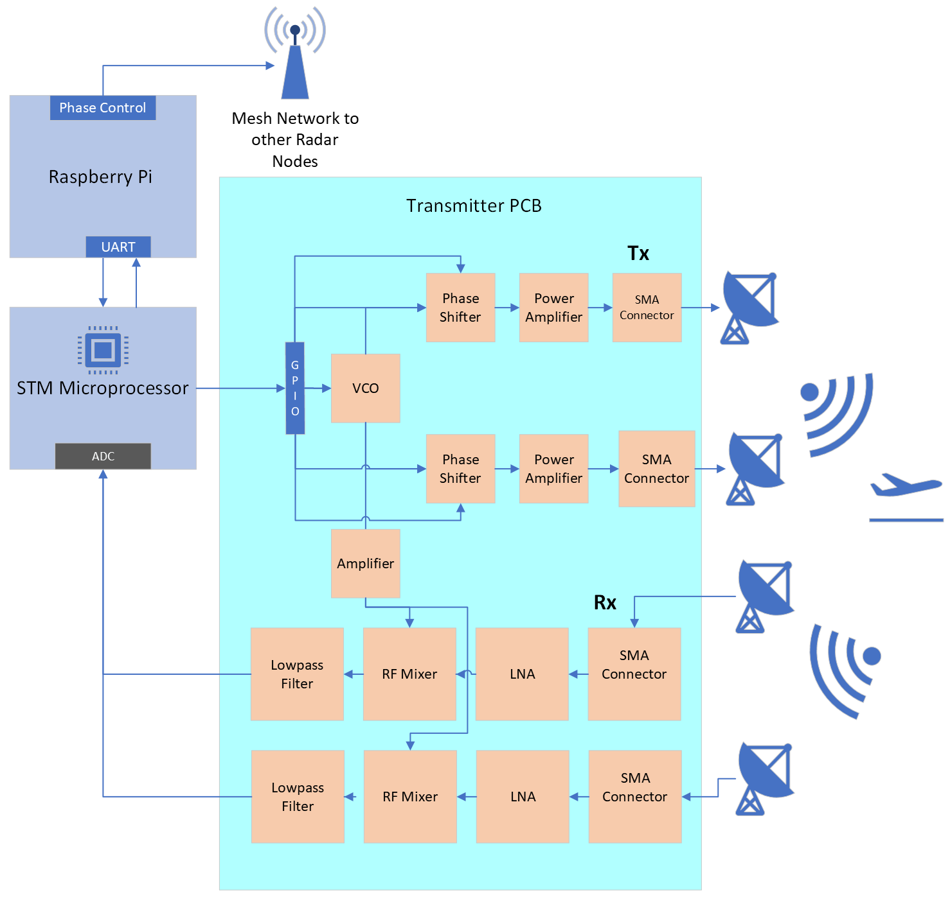
\includegraphics{Diagrams/overview.png}}
\caption{Architecture Overview}
\label{img:projoverview}
\end{figure}

In this chapter, we will go through the architecture of the PCB and show what parts we picked and what purposes they serve.
Figure \ref{img:projoverview} shows the overall architecture of the project.

\section{Voltage Controlled Oscillator (VCO)}
The first step in creating a radar is signal synthesis. You essentially need to create an alternating current signal that can
go through your antenna and radiate out into the air. To reiterate from Chapter \ref{Radar Theory}, higher frequency signals are
important for a better radar resolution, and so it is desired to have a signal that is high in frequency. Naively, at the
beginning of this project we thought we could use a 16 bit DAC to synthesize our signal but after finding out its max clock rate 
was 1 MHz, we realized a DAC was not fit for this. All we needed was something that could create a simple sinusoid at a very
high frequency.

Voltage Controlled Oscillators (VCO) do just this. They take in a "tuning voltage" which corresponds to a certain frequency
of sinusoid which it will output. The circuitry for this is beyond me, but for a good overall guide on VCOs you can check out
DigiKey's article \href{https://www.digikey.com/en/articles/the-basics-of-voltage-controlled-oscillators-vcos}{here}.

Now that we knew how to synthesize our signal, it was important to find a good VCO that had a high output bandwidth. Whatever
bandwidth the VCO has will impact what parts we can get in the other stages of the RF chain since these must be within the VCOs
operating regions. 

\begin{figure}[H]
    \centering
    \scalebox{.7}{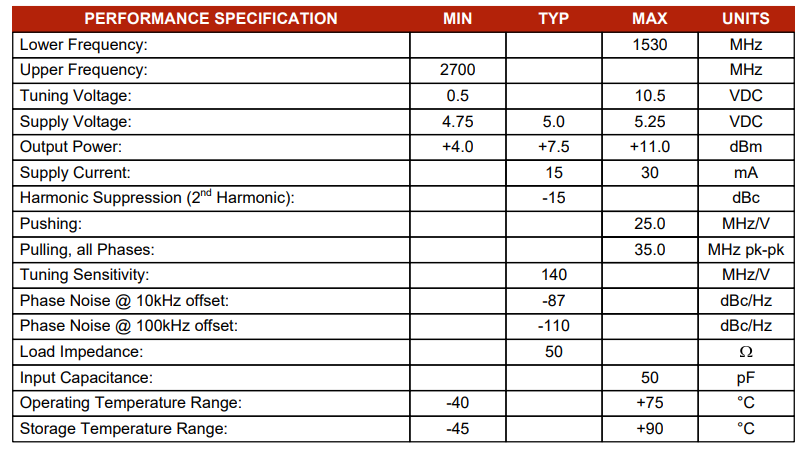
\includegraphics{DatasheetImages/vcotable.png}}
    \caption{VCO Datasheet Table}
    \label{img:vcotable}
\end{figure}
\begin{figure}[H]
    \centering
    \scalebox{.7}{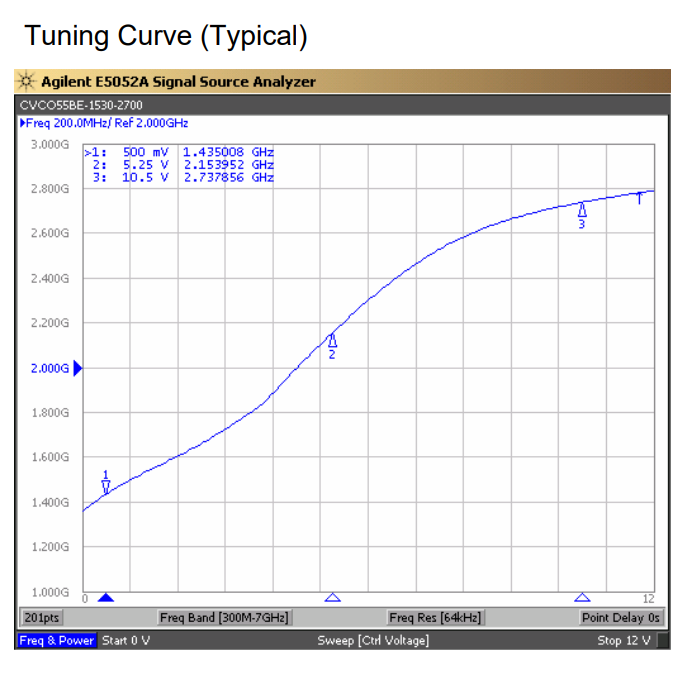
\includegraphics{DatasheetImages/vcotuningtable.png}}
    \caption{Tuning Voltage Graph}
    \label{img:tuninggraph}
\end{figure}

We chose a VCO from Crystek which can be found on Digikey \href{https://www.digikey.com/en/products/detail/crystek-corporation/CVCO55BE-1530-2700/1644030}{here}.
Looking at the specifications table in Figure \ref{img:vcotable}, some good things to look for are first and foremost the frequency
range of the part. It goes from about 1.5-2.7 GHz, which is a pretty wide range and would support a lot of other parts as it also
covers the Wi-Fi band. The second thing to look for is output power. The output power can be a constraint for other parts, since they
might have a absolute limit on their input power, and it is useful to know the output power for finding out how strong your signal will be
once it propogates out of your antenna. Here we can see the output power is around 7.5 dBm, and this will be split four ways. 
Decibels are a logarithmic scale, so we cannot just divide by four but instead use a decibel calculator like \href{https://noisetools.net/decibelcalculator}{this one}.

Now, another key metric is the tuning voltage. Luckily, this Crystek provides a tuning voltage graph found in Figure \ref{img:tuninggraph}
that shows us how the output frequency changes with changes in the tuning voltage. One observation is that it is not linear, meaning
our ramp voltage will not result in a true linear ramp in frequency. Another observation is that our chosen frequency of 1.8 GHz is
around 3.5 volts following the graph. Our STM board that will generate the ramp voltage can by default only go to 3.3 volts, but we
found a workaround to go to 5 volts which allowed us to stick with our decided center frequency.

\section{Power Divider}
As mentioned before, we want to divide the VCO's signal four ways because want it to go to two phase shifters, and two mixers.
At first we thought it was as simple as having one wire split into four, but as we will go over in Chapter \ref{PCB}, impedence
matching is very important in RF circuits. To put it simply, impedance matching ensures that no power is reflected, and this is
important because reflected power means distortions in the signal and power loss. That means we needed a power splitter meant for
splitting an RF signal without causing reflected power. There is not much of note with the part we used which can be found 
\href{https://www.mouser.com/ProductDetail/Mini-Circuits/WP4P1%2B?qs=Imq1NPwxi77kWybHhilv%2Fg%3D%3D}{here}. The main thing is that
it contains the frequency of 1.8 GHz we want to use.

\section{Phase Shifter}
Two of the power dividers split paths will go into phase shifters. The phase shifters are used to make our phased array
of antennas as explained in Chapter \ref{Radar Theory}. They are able to change the phase (add time delay), to the signal 
so that when they propogate through the air they can construct and destruct. The phase shifters we chose can be found
\href{https://www.digikey.com/en/products/detail/psemi/PE44820B-X/5822957}{here}. These are digital phase shifters that have 256
different phases it can apply to the signal. They have a parallel or serial interface we can use to transmit 8 bit words That
will alter the phase of our signal. The interface and its timing diagrams will be explained more in detail in Chapter \ref{Digital Processing}.
All we need to know is that the bandwidth that the chip supports contains 1.8 GHz.

\section{Power Amplifier}
\begin{figure}[H]
  \centering
  \scalebox{.6}{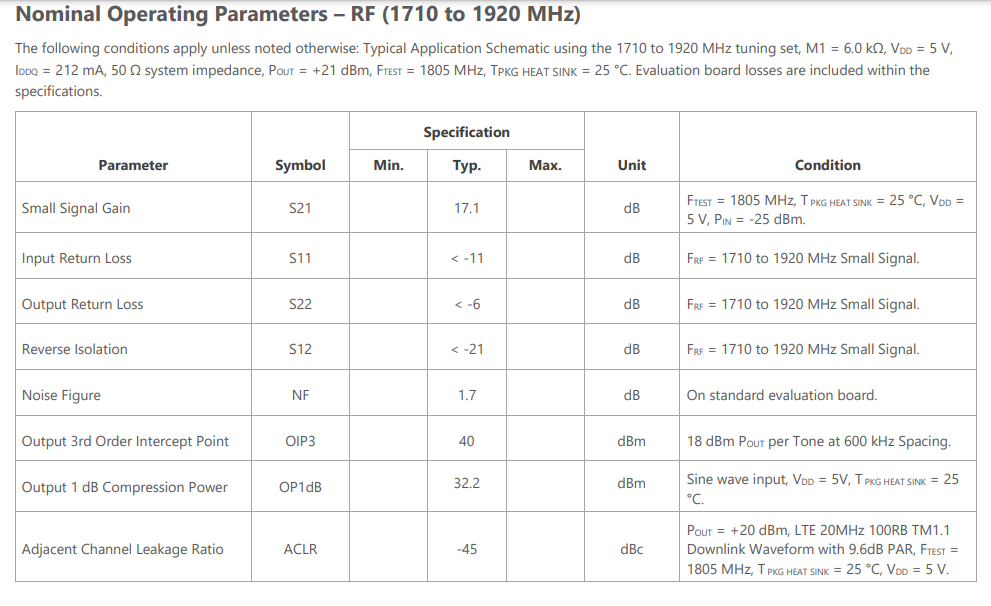
\includegraphics{DatasheetImages/poweramptable.png}}
  \caption{Power Amplifier Table}
  \label{img:poweramptable}
\end{figure}
At this point after the VCO and phase shifter, we want the RF signal to propogate through the air. However, according to the
radar range equation the power of the signal when attenuating through the air attenuates at a power of four which is a lot.
Therefore, we need to make sure our signal is powerful enough to go pretty far. So, we use an RF power amplifier to amplify the
signal. We chose a part from GuerillaRF which can be found \href{https://www.mouser.com/ProductDetail/Guerrilla-RF/GRF5112?qs=ulEaXIWI0c%252Bti188Qa1Now%3D%3D}{here}.
Looking at the table in Figure \ref{img:poweramptable}, we can see some key metrics when looking at power amplifiers. First,
of course we want to make sure it has a bandwidth that supports our chosen frequency of 1.8 GHz. Second, we want to look at the
small-signal gain and Output 1 dB Compression Point or OP1dB. The small-signal gain is the ideal gain that can be reached with a 
low power signal, and is listed as 17.1 dB. The OP1dB is a metric we did not know about and were thankful to find it. With most amplifiers,
gain operates linearly meaning whatever power your input signal is you just add the gain of the amplifier and this will be the resulting power of the signal.
However, at a certain point the amplifier saturates and does not operate linearly anymore, and will essentially cap-off its gain at
the OP1dB limit. For example, with the OP1dB being 32.2 dB, if I input a signal that was 30 dB I would expect a resulting signal of
47.1 dB but this would not be the case. The amplifier ceases to operate linearly after the 32.2 dB mark, and will both distort the signal
and output something weaker than expected. A lot of amplifiers will boast a high gain but have a low OP1dB, so this is definitely something to check for.

\section{Low Noise Amplifier}
\begin{figure}[H]
  \centering
  \scalebox{.7}{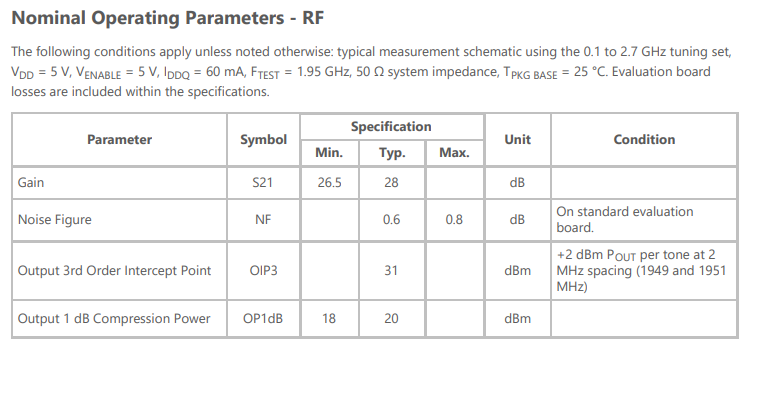
\includegraphics{DatasheetImages/lnatable.png}}
  \caption{Low-Noise Amplifier Table}
  \label{img:lnatable}
\end{figure}

This is the first part that will be placed in the receiver RF chain. According to the Friis equation in Chapter \ref{Radar Theory},
the first stage in the receiver RF chain matters a lot for the noise figure of your system. Therefore, we wanted to find a part
with a low noise figure and high gain, as this will impact our SNR the most. Low noise amplifiers are made for this exact purpose,
where they amplify a small signal with very low noise. The part we chose was \href{https://www.mouser.com/ProductDetail/Guerrilla-RF/GRF2133W?qs=ulEaXIWI0c%2FXgAPwqRmr2A%3D%3D}{this},
which is made by GuerillaRF. By examining the table in Figure \ref{img:lnatable}, we can see that it has a gain of 28 dB,
and a noise figure of .6 dB. We also can look at the OP1dB which has a figure of 20 dB. Since the LNA will be amplifying a signal
straight from an antenna, the signal will be super weak and there is a low likelihood it will reach the OP1dB.

\section{Mixer/LO Amp}
\begin{figure}[H]
  \centering
  \scalebox{.7}{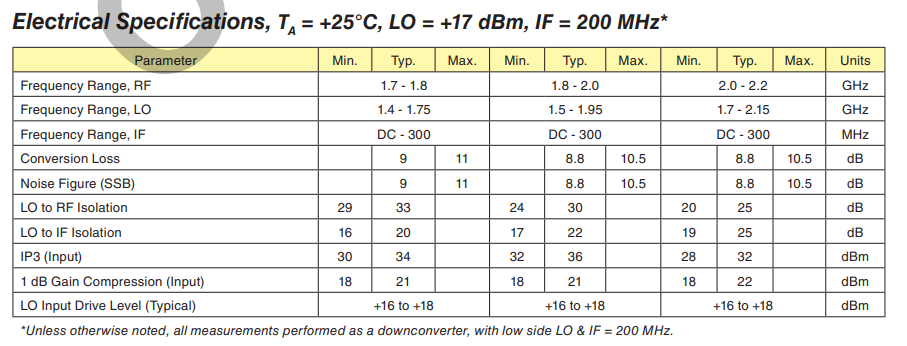
\includegraphics{DatasheetImages/mixertable.png}}
  \caption{Mixer Table}
  \label{img:mixertable}
\end{figure}
\begin{figure}[H]
  \centering
  \scalebox{.7}{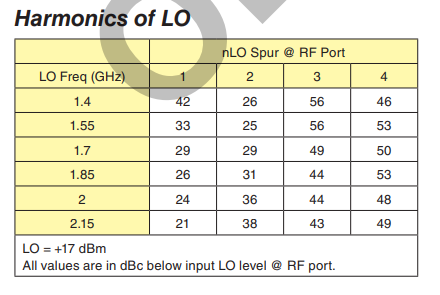
\includegraphics{DatasheetImages/mixerharmonics.png}}
  \caption{Mixer Harmonics Table}
  \label{img:mixerharmonics}
\end{figure}

Now that our received signal is amplified we must down-convert it in order to sample and process it. The process for doing
this is called heterodyning or mixing, and the theory behind this can be found in detail in Chapter \ref{Radar Theory}. 
A mixer has three ports, the local oscillator, RF signal, and output. The local oscillator and RF signal are multiplied
to produce the sum and difference of the LO and RF signals on the output port. We are mainly interested in the difference,
also called the Intermediate Frequency (IF) since it is a low frequency and can be sampled easily.
In our case, we take a copy of the VCO as the local oscillator and then mix this with the amplified return signal 
to produce our intermediate frequency. To achieve this, we used a discontinued mixer from Analog Devices which
can be found \href{https://www.arrow.com/en/products/hmc400ms8etr/analog-devices}{here}. 
Looking at the mixer's specifications table in Figure \ref{img:mixertable}, we can 
see some new properties. The conversion loss is the output IF power delivered minus the available RF input signal power. The
LO to RF Isolation is how much of the local oscillator signal leaks into the RF port, and the LO to IF Isolation is how much
the local oscillator signal leaks into the output port. This is a passive component, meaning it does not require power and
solely operates off the power of the LO and RF signals. Therefore we see in the table that the LO Input must be 16-18 dBm to drive
the mixer. Essentially the local oscillator powers the mixer, and its harmonics will therefore be prominent in the IF port due to
leakage. We can see in Figure \ref{img:mixerharmonics} that at 1.85 GHz the manufacturer tells us the strength of LO harmonics 
up to the fourth order. At the top it says spur which means spurious (unwanted) outputs due to the nonlinearity of the mixer.
Essentially this table tells us that there will be unwanted spectral components in the output, which is something we did not
pay enough attention to and will discuss in Chapter \ref{Issues}.
\begin{figure}[H]
  \centering
  \scalebox{.7}{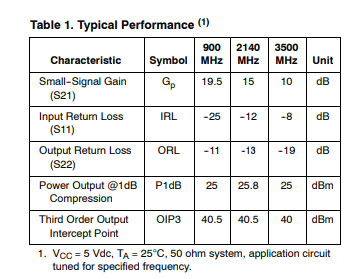
\includegraphics{DatasheetImages/loamptable.png}}
  \caption{LO Amp Table}
  \label{img:loamptable}
\end{figure}

As we said before, the mixer is a passive component which is driven by the LO which needs a power level of 16-18 dBm.
After splitting our VCO's output four ways, we have about a ~2 dBm signal that we must amplify. So, we chose an RF broadband
amplifier from NXP which can be found \href{https://www.digikey.com/en/products/detail/nxp-usa-inc/MMG3014NT1/1971761}{here}. As
we can see in Figure \ref{img:loamptable}, the amp has a gain of around 15 dB for our frequency and an OP1dB of 25.8 dB which is
a lot of headroom.

\section{IF Amplifiers and Filters}
Now, our return signal has been downconverted, but the power of that signal is very weak. As well as this, there are unwanted
spectral components in that signal that are bi-products of the mixer that we need to get rid of. This means we need amplifiers and
filters to make our signal ready to be sampled and processed in the microcontroller. First we used a super simple op-amp
that served as a voltage follower which can be found \href{https://www.digikey.com/en/products/detail/microchip-technology/MCP6001UT-I-OT/562450}{here}.
This was used to create a virtual ground for our biasing. Then we use a dual channel op-amp from TI for our variable gain
amplifier which can be found \href{https://www.mouser.com/ProductDetail/Texas-Instruments/LM2904DR?qs=5BZzbFV4k2vkQqOl3Q8qPg%3D%3D}{here}.

\begin{figure}[H]
  \centering
  \scalebox{.7}{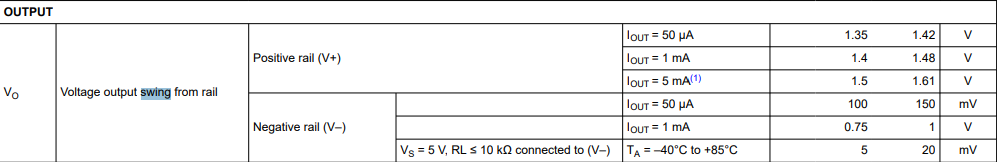
\includegraphics{DatasheetImages/outputswing.png}}
  \caption{Output Swing Characteristics}
  \label{img:outputswing}
\end{figure}

Honestly, when selecting parts we figured all operational amplifiers just acted the same way. However, after printing and manufacturing
we ran into problems which will be discussed in Chapter \ref{Issues} that could have been remedied if we paid more attention to
the Op-Amps we were using. The main problem is that these operational amplifiers are not "Rail-to-Rail".
While rail-to-rail amplifiers guarantee that they do not saturate until the positive and negative voltages you've supplied it,
other amplifiers have what is called voltage swing. As we can see in Figure \ref{img:outputswing}, the range of voltage
that the operational amplifier can achieve is not its rails, but specifies how much lower than its rail it will be. This is 
something to look out for when selecting an Op-Amp.

\begin{figure}[H]
  \centering
  \scalebox{.7}{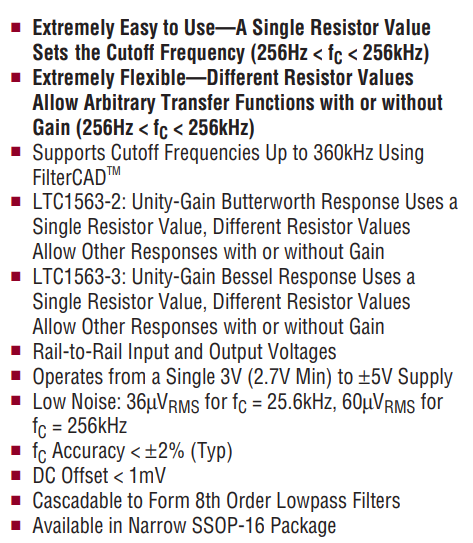
\includegraphics{DatasheetImages/filterspecs.png}}
  \caption{Filter Features}
  \label{img:filterspecs}
\end{figure}

After amplifying the signal, we wanted to filter out unwanted spectral components by using a strong filter. Instead of designing
this ourselves, we decided to use a 4th Order LPF which can be found \href{https://www.digikey.com/en/products/detail/analog-devices-inc/LTC1563-2IGN-PBF/962958}{here}.
By looking at Figure \ref{img:filterspecs}, we can see that this is an integrated circuit with a flexible cutoff frequency.
It also says that it is a rail-to-rail input and output circuit, which is an important feature to note as discussed with the amplifiers.
A fourth order filter just means that this filter has four filters with the same cutoff frequency cascaded upon each other, which
yields a steeper frequency response and attenuates are unwanted signals further.
\chapter{PCB
\index{Chapter!PCB}
\index{PCB}
\label{PCB}}
\chapter{Digital Processing
\index{Chapter!Digital Processing}
\index{Digital Processing}
\label{Digital Processing}}
\chapter{Networking
\index{Chapter!Networking}
\index{Networking}
\label{Networking}}


\chapter{Results
\index{Chapter!Results}
\index{Results}
\label{Results}}
\chapter{Issues
\index{Chapter!Issues}
\index{Issues}
\label{Issues}}

%\bibliography{bibfile}
%\bibliographystyle{unsrt}
%\bibliographystyle{IEEEtran}

%% Initial version by Darian Muresan, Ph.D.
% Edit and adjust as needed.

\documentclass[12pt]{cornell}

% add index support
\makeindex

% graphing programs
\usepackage{color}
\usepackage{psfrag}
\usepackage{verbatim}
\usepackage{fancyhdr}
\usepackage{minted}
%\usepackage{titlesec}
\usepackage{fancyvrb} 
% hyperlink programs
\usepackage[luatex, 
breaklinks=true, 
colorlinks=true,
citecolor=blue,
linkcolor=blue,
menucolor=black,
pagecolor=black,
urlcolor=blue
]{hyperref} % links in pdf
%\usepackage[colorlinks]{hyperref} % links in dvi
\usepackage{listings}
\usepackage{amsfonts} 
\usepackage{amssymb} 
%\usepackage{tabto}

\usepackage{tabularx,colortbl}
\usepackage[chapter]{algorithm} 
\usepackage{algorithmic} 
\usepackage{blindtext}
\usepackage{imakeidx}

% for electronics:
\usepackage[american]{circuitikz}

\definecolor{DarkGreen}{rgb}{0,0.6,0}
\definecolor{mygreen}{rgb}{0,0.6,0}
\definecolor{mygray}{rgb}{0.5,0.5,0.5}
\definecolor{mymauve}{rgb}{0.58,0,0.82}

\usepackage{tocloft}
\usepackage{amsmath}
\usepackage{tcolorbox}
\usepackage{enumitem}
\usepackage{longtable}
%\usepackage{textcomp}
\usepackage{txfonts}

%part for \part titles
%chap for \chapter titles
%sec for \section titles
%subsec for \subsection titles
%subsubsec for \subsubsection titles
%para for \paragraph titles
%subpara for \subparagraph titles
%fig for figure \caption titles
%subfig for subfigure \caption titles
%tab for table \caption titles
%subtab for subtable \caption titles

% update chapter number spacing
\setlength{\cftchapnumwidth}{2em}
\setlength{\cftsecnumwidth}{2.5em}
\setlength{\cftsubsecnumwidth}{3.5em}
\setlength{\cftsubsubsecnumwidth}{4.5em}

\addtolength{\cftsecindent}{0.5em}
\addtolength{\cftsubsecindent}{0.5em}
\addtolength{\cftsubsubsecindent}{0.5em}

%\titlespacing*{\chapter}{0pt}{-50pt}{20pt}
%\titleformat{\chapter}[display]{\normalfont\huge\bfseries}{\chaptertitlename\ 
%\thechapter}{20pt}{\Huge}
%\pagestyle{fancy}
%\pagestyle{cornell}
%
%\rhead{F054-021-0172}
%\chead{Nonlinear Enhancement of Visual Target Detection (AF05-T021)}
%\lhead{GSTI}
%\lfoot{\scriptsize Use or disclosure of data on this page is subject
%to the restriction on the title page of this proposal.}
%\cfoot{}
%\rfoot{\thepage}

\newfont{\Bp}{msbm10}
\newfont{\BpBig}{msbm10 scaled\magstep2}
\newfont{\Sc}{eusm10}
\newfont{\ScBig}{eusm10 scaled\magstep3}
\newfont{\Fr}{eufm10}
\newfont{\FrBig}{eufm10 scaled\magstep1}

% some commands:
\newcommand{\dxi}{{\tt m\_xDeltaInput}}
\newcommand{\dyi}{{\tt m\_yDeltaInput}}
\newcommand{\dci}{{\tt m\_cDeltaInput}}
\newcommand{\dxo}{{\tt m\_xDeltaOutput}}
\newcommand{\dyo}{{\tt m\_yDeltaOutput}}
\newcommand{\dco}{{\tt m\_cDeltaOutput}}
\newcommand{\ttf}[1]{{\tt #1}}
\newcommand{\tbl}[2]{{\begin{tabular}{c} #1 \\ #2 \end{tabular}}}

\newcommand{\urltwo}[2]{\mbox{\href{#1}{\tt #2}}}
\newcommand{\qnorm}[1]{\|#1\|_{\bQ}}
\newcommand{\qdot}[2]{\lrb #1, #2 \rrb_{\bQ}}
\newcommand{\kdot}[2]{\lrb #1, #2 \rrb_{\bf k}}
\newcommand{\tdot}[2]{\lrb #1, #2 \rrb}
\newcommand{\mydiff}[2]{\lrb #1 - #2 \rrb}
\newcommand{\lena}{\textit{lena}}
\newcommand{\barb}{\textit{barbara}}
\newcommand{\boat}{\textit{boat}}
\newcommand{\leaves}{\textit{leaves}}
\newcommand{\rings}{\textit{rings}}
\newcommand{\treg}{\textit{train region}}
\newcommand{\dreg}{\textit{denoise region}}
\newcommand{\oreg}{\textit{overlap region}}
\newcommand{\sil}{\sigma_l^2}
\newcommand{\sn}{\sigma^2}
\newcommand{\bn}{{\mbox{\bf \FrBig N}}}
\newcommand{\n}{\mbox{\Fr N}}
%\newcommand{\bn}{\bf N}
%\newcommand{\n}{N}
\newcommand{\bY}{\textbf{Y}}
\newcommand{\bX}{\textbf{X}}
\newcommand{\bb}{\textbf{b}}
\newcommand{\bu}{\textbf{u}}
\newcommand{\bv}{\textbf{v}}
\newcommand{\by}{\textbf{y}}
\newcommand{\bx}{\textbf{x}}
\newcommand{\be}{\textbf{e}}
\newcommand{\bz}{\textbf{z}}
\newcommand{\bs}{\textbf{s}}
\newcommand{\bw}{\textbf{w}}
\newcommand{\bQ}{\textbf{Q}}
\newcommand{\bphi}{\textbf{$\phi$}}
\newcommand{\lsb}{\left[}
\newcommand{\rsb}{\right]}
\newcommand{\lrb}{\left(}
\newcommand{\rrb}{\right)}
\newcommand{\lcb}{\left\{}
\newcommand{\rcb}{\right\}}
\newcommand{\R}{\mbox{\BpBig R}}
\newcommand{\F}{{\cal F}}
\newcommand{\Fk}{\mbox{\Sc F}}
\newcommand{\bQF}{\textbf{Q}_{\mbox{\Sc F}}}
\newcommand{\N}{{\cal N}}
\newcommand{\xlz}{X_l(z)}
\newcommand{\xhz}{X_h(z)}
\newcommand{\xz}{X(z)}
\newcommand{\pr}{ perfect reconstruction }
\newcommand{\smb}{Smith-Barnwell }
\newcommand{\xw}{X(e^{j\omega})}
\newcommand{\xmw}{X(-e^{j\omega})}
\newcommand{\dw}{D(e^{j\omega})}
\newcommand{\dmw}{D(-e^{j\omega})}
\newcommand{\ew}{E(e^{j\omega})}
\newcommand{\emw}{E(-e^{j\omega})}
\newcommand{\fw}{F_0(e^{j\omega})}
\newcommand{\fmw}{F_0(-e^{j\omega})}
\newcommand{\hoz}{H_1(z)}
\newcommand{\hzz}{H_0(z)}
\newcommand{\goz}{G_1(z)}
\newcommand{\gzz}{G_0(z)}
\newcommand{\hzw}{H_{0}(e^{j\omega})}
\newcommand{\hzmw}{H_{0}(-e^{j\omega})}
\newcommand{\hzcw}{H_{0}(e^{-j\omega})}
\newcommand{\how}{H_1(e^{j\omega})}
\newcommand{\homw}{H_1(-e^{j\omega})}
\newcommand{\gzw}{G_0(e^{j\omega})}
\newcommand{\gzmw}{G_0(-e^{j\omega})}
\newcommand{\gow}{G_1(e^{j\omega})}
\newcommand{\gomw}{G_1(-e^{j\omega})}
\newcommand{\wl}{e^{-jwL}}
\newcommand{\aqua}{\textit{AQua with OR }}
\newtheorem{theorem}{Theorem}
\newtheorem{lemma}{Lemma}
\newtheorem{corollary}{Corollary}
\newtheorem{claim}{Claim}
\newtheorem{definition}{Definition}
\newenvironment{proof}{\noindent{\em Proof.}}{\ \hfill Q.E.D.}
%\newtheorem{moduleCount}{L}
\newcommand*{\labelfile}[1]{%
  \label{file:#1}%
}

\lstset{ %
  backgroundcolor=\color{white},   % choose the background color; you must add \usepackage{color} or \usepackage{xcolor}
  basicstyle=\footnotesize,        % the size of the fonts that are used for the code
  breakatwhitespace=false,         % sets if automatic breaks should only happen at whitespace
  breaklines=true,                 % sets automatic line breaking
  captionpos=b,                    % sets the caption-position to bottom
  commentstyle=\color{DarkGreen},    % comment style
  deletekeywords={...},            % if you want to delete keywords from the given language
  escapeinside={\%*}{*)},          % if you want to add LaTeX within your code
  extendedchars=true,              % lets you use non-ASCII characters; for 8-bits encodings only, does not work with UTF-8
  %frame=single,                   % adds a frame around the code
  keepspaces=true,                 % keeps spaces in text, useful for keeping indentation of code (possibly needs columns=flexible)
  keywordstyle=\color{blue},       % keyword style
  language=C++,                    % the language of the code
  morekeywords={*,...},            % if you want to add more keywords to the set
  numbers=left,                    % where to put the line-numbers; possible values are (none, left, right)
  numbersep=5pt,                   % how far the line-numbers are from the code
  numberstyle=\tiny\color{mygray}, % the style that is used for the line-numbers
  rulecolor=\color{black},         % if not set, the frame-color may be changed on line-breaks within not-black text (e.g. comments (green here))
  showspaces=false,                % show spaces everywhere adding particular underscores; it overrides 'showstringspaces'
  showstringspaces=false,          % underline spaces within strings only
  showtabs=false,                  % show tabs within strings adding particular underscores
  stepnumber=1,                    % the step between two line-numbers. If it's 1, each line will be numbered
  stringstyle=\color{mymauve}     % string literal style
  %tabsize=2,                      % sets default tabsize to 2 spaces
  %caption=\lstname                % show the filename of files included with \lstinputlisting; also try caption instead of title
}

% Uncomment draftcopy to get the word DRAFT boldly across the first page
%   By the way, xdvi won't show it but it will come out when you print
%\usepackage[light,all]{draftcopy}		% DRAFT on first page
%\draftcopySetGrey{.97}
%\draftcopyName{Confidential}{150}
%\draftcopFirstPage{1}

% Uncomment drafthead to get the date and DRAFT in the header of pages
% that are normallly numbered on the top, pages 2-n of each chapter for example
% This doesn't work with centered page numbers: \pagestyle{cornellc}
%\usepackage{drafthead}

% Including selective chapters:
% use this to selectively process chapters, etc.  Put a % in front of
% the sections that you don't want done this time.  Includes are
% used instead of \input so that LaTeX will keep track of chapters and
% pages without processing everything.  Don't let any spaces creep in
% around the words or it will not work!


\includeonly{
prologue,
manIntroduction,
manProjectDescription,
manResources,
manRadarTheory,
manPartSelection,
manPCB,
manDigitalProcessing,
manNetworking,
manResults,
manIssues
}

\makeindex

\begin{document}

\pagenumbering{roman}
\singlespacing
% File: prologue.tex
% Thesis prologue:  Title page, acknowledgements, table of contents,
% list of figures, and list of tables.
%
% this file is to be \include'd after the \begin{document}

% Cornell-style title page
\begin{titlepage}
        \title{Mithril - FMCW Radar}
        \author{Tomas Esson, Ajay Thakkar, Juan Jimenez \\ tesson@stevens.edu, athakka5@stevens.edu, jjimene6@stevens.edu }
        \conferraldate{}{\today} \maketitle
\end{titlepage}

% Copyright page
%\begin{copyrightpage}
\makecopyright
%\end{copyrightpage}

% Abstract: the abstract body is pulled from the file abstract.tex;
%  the title is pulled from the \title command in the titlepage section

% Biographical information pulled from file bio.tex
%\begin{biosketch} \input bio \end{biosketch}

% Dedication (optional):  pulls information from file dedication.tex
%\begin{dedication} 
%\input dedicate 
%\end{dedication}

% Acknowledgements:  pulls information from file acknow
%\begin{acknowledgements} \input acknow \end{acknowledgements}

% Table of contents
\contentspage

% If you have no tables or figures put a % in front of the list page line
% List of tables
\tablelistpage

% List of figures
\figurelistpage



\setcounter{page}{1}        % set page counter
\pagenumbering{arabic}      % set page number style
\pagestyle{fancy}         % top right page numbers
%\pagestyle{cornell}
%\pagestyle{cornellc}       % centered page numbers, disables drafthead

\renewcommand{\chaptermark}[1]{\markboth{#1}{}}
\renewcommand{\sectionmark}[1]{\markright{#1}{}}

\fancyhead{} % clear all fields

\lhead{Chapter \thechapter}
%\lhead{\thechapter}
\chead{\leftmark}
\rhead{\thepage}


\lfoot{Chapter \thechapter}
\cfoot{\copyright Stevens -- \today \mbox{} -- FPGA Radio Receiver/Transmitter}
\rfoot{\thepage}

\renewcommand{\headrulewidth}{0.4pt}
\renewcommand{\footrulewidth}{0.4pt}

%\rhead{F054-021-0172}
%\chead{Nonlinear Enhancement of Visual Target Detection (AF05-T021)}
%\lhead{GSTI}
%\lfoot{\scriptsize Use or disclosure of data on this page is subject
%to the restriction on the title page of this proposal.}
%\cfoot{}
%\rfoot{\thepage}


\singlespacing
\chapter{Introduction 
\index{Chapter!Introduction}
\index{Introduction}
\label{Introduction}}

The following includes small biographies on all the authors as well as their research interests and projects.

\section*{Authors' Biographies}
\subsection*{Ajay Thakkar}
\textbf{Ajay Thakkar} Ajay Thakkar is a junior majoring in Computer Engineering. He is interested in signal processing and lower level coding. Below you can find his GitHub: \url{https://github.com/athakkar2}.

\subsection*{Tomas Esson}
\textbf{Tomas Esson} is an aspiring Computer Engineering at Stevens Institute of technology. He is an avid surfer and enjoys elegant math proofs. Currently pursuing interests in computer chip design, digital systems implementation, mathematical optimization of computer chips, and electrical engineering. 

\subsection*{Juan Jimenez}
\textbf{Juan Jimenez} is a Junior Computer Engineering student at the Stevens Institute of technology. Interested in the intersection between Artificial Intelligence, embedded electronics, and software engineering. To see more projects visit the following GitHub link: \url{https://github.com/jjimene1}  
\chapter{Project Description 
\index{Chapter!Project Description}
\index{Project Description}
\label{Project Description}}
\begin{figure}[H]
  \centering
  \begin{tikzpicture}[node distance = 2cm, auto]
      % Define block styles
      \tikzstyle{block} = [rectangle, draw, fill=blue!20, 
          text width=5em, text centered, rounded corners, minimum height=4em]
      \tikzstyle{line} = [draw, ->]
  
      % Place nodes
      \node [block] (mithril) {Mithril};
      \node [block, below of=mithril, node distance=4cm] (radar) {FMCW Radar};
      \node [block, left of=radar, node distance=4cm] (processing) {Digital Processing};
      \node [block, right of=radar, node distance=4cm] (networking) {Distributed Networking};
      \node [block, below of=processing, node distance=2cm] (STM) {STM MC and Python};
      \node [block, below of=radar, node distance=2cm] (ORCad) {Cadence ORCad};
      \node [block, below of=networking, node distance=2cm] (pi) {Raspberry Pi and MQTT};
      % Draw edges
      \path [line] (mithril) -- (radar);
      \path [line] (mithril) -- (processing);
      \path [line] (mithril) -- (networking);
      \path [line] (radar) -- (ORCad);
      \path [line] (processing) -- (STM);
      \path [line] (networking) -- (pi);
  \end{tikzpicture}
  \caption{Flowchart of the Mithril system}
  \label{fig:mithril_flowchart}
  \end{figure}
Mithril is a nodal FMCW radar system that incorporates traditional FMCW radar,
digital processing, edge computing, and distributed networking. The initial idea of this 

As can be seen in Figure \ref{fig:mithril_flowchart},
the radar was designed as a standalone PCB in ORCad, digital processing was handled by
STM microcontrollers, and distributed networking is done via Raspberry Pi's and the MQTT protocol.
All of these components were designed, engineered, and interfaced from scratch with a limited budget
of 2000 dollars.

\section{}
The heart of the project is a standalone PCB capable of FMCW radar.
\chapter{Resources
\index{Chapter!Resources}
\index{Resources}
\label{Resources}}
\chapter{Radar Theory
\index{Chapter!Radar Theory}
\index{Radar Theory}
\label{Radar Theory}}

\section{Getting Started}



include the benefits of using higher frequency signals

heterodyning
\chapter{Part Selection
\index{Chapter!Part Selection}
\index{Part Selection}
\label{Part Selection}}

\begin{figure}[H]
  \centering
  \scalebox{.8}{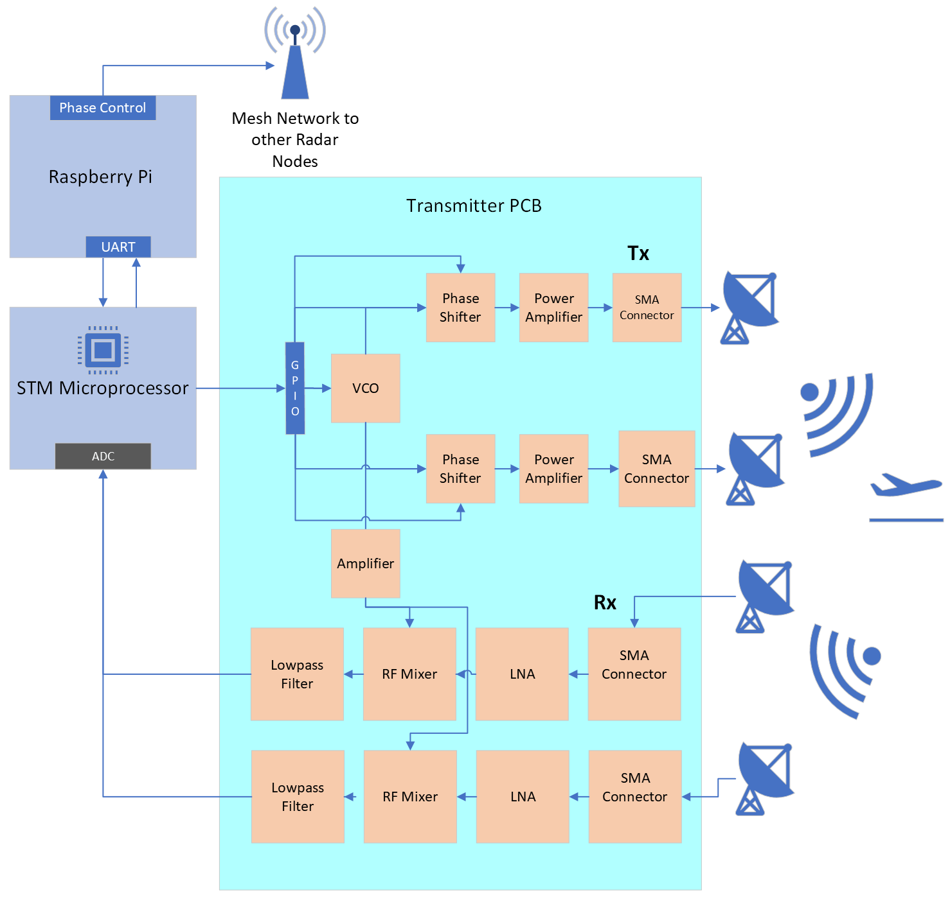
\includegraphics{Diagrams/overview.png}}
\caption{Architecture Overview}
\label{img:projoverview}
\end{figure}

In this chapter, we will go through the architecture of the PCB and show what parts we picked and what purposes they serve.
Figure \ref{img:projoverview} shows the overall architecture of the project.

\section{Voltage Controlled Oscillator (VCO)}
The first step in creating a radar is signal synthesis. You essentially need to create an alternating current signal that can
go through your antenna and radiate out into the air. To reiterate from Chapter \ref{Radar Theory}, higher frequency signals are
important for a better radar resolution, and so it is desired to have a signal that is high in frequency. Naively, at the
beginning of this project we thought we could use a 16 bit DAC to synthesize our signal but after finding out its max clock rate 
was 1 MHz, we realized a DAC was not fit for this. All we needed was something that could create a simple sinusoid at a very
high frequency.

Voltage Controlled Oscillators (VCO) do just this. They take in a "tuning voltage" which corresponds to a certain frequency
of sinusoid which it will output. The circuitry for this is beyond me, but for a good overall guide on VCOs you can check out
DigiKey's article \href{https://www.digikey.com/en/articles/the-basics-of-voltage-controlled-oscillators-vcos}{here}.

Now that we knew how to synthesize our signal, it was important to find a good VCO that had a high output bandwidth. Whatever
bandwidth the VCO has will impact what parts we can get in the other stages of the RF chain since these must be within the VCOs
operating regions. 

\begin{figure}[H]
    \centering
    \scalebox{.7}{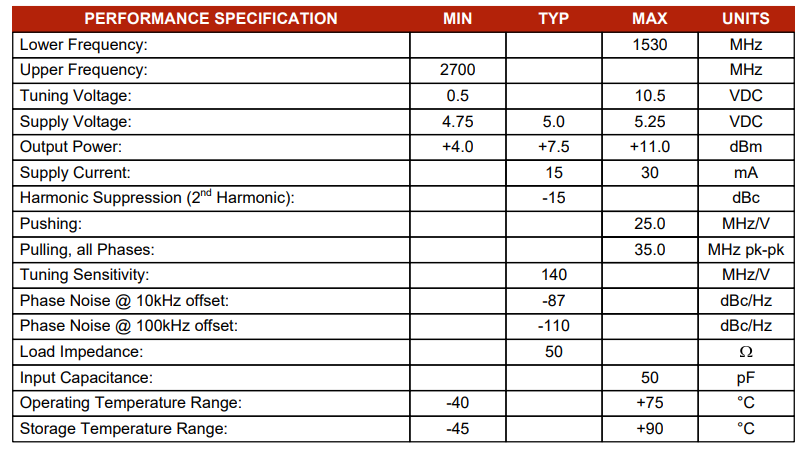
\includegraphics{DatasheetImages/vcotable.png}}
    \caption{VCO Datasheet Table}
    \label{img:vcotable}
\end{figure}
\begin{figure}[H]
    \centering
    \scalebox{.7}{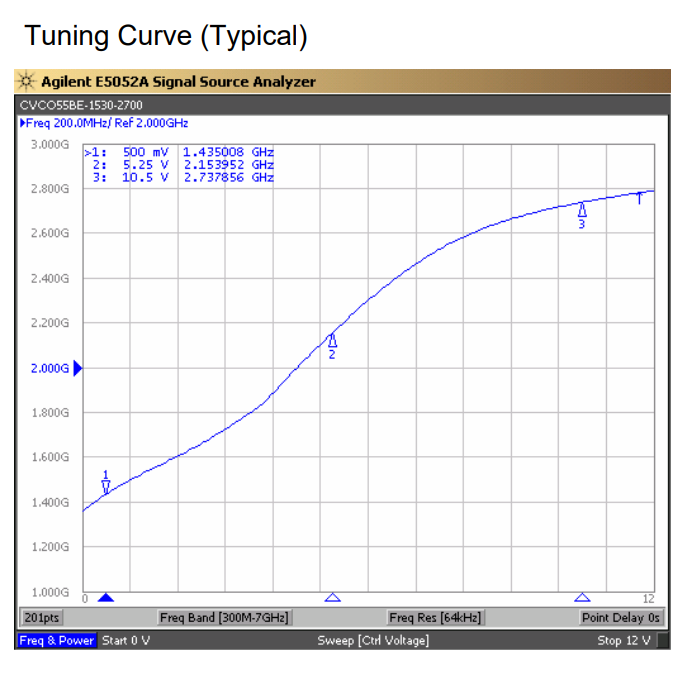
\includegraphics{DatasheetImages/vcotuningtable.png}}
    \caption{Tuning Voltage Graph}
    \label{img:tuninggraph}
\end{figure}

We chose a VCO from Crystek which can be found on Digikey \href{https://www.digikey.com/en/products/detail/crystek-corporation/CVCO55BE-1530-2700/1644030}{here}.
Looking at the specifications table in Figure \ref{img:vcotable}, some good things to look for are first and foremost the frequency
range of the part. It goes from about 1.5-2.7 GHz, which is a pretty wide range and would support a lot of other parts as it also
covers the Wi-Fi band. The second thing to look for is output power. The output power can be a constraint for other parts, since they
might have a absolute limit on their input power, and it is useful to know the output power for finding out how strong your signal will be
once it propogates out of your antenna. Here we can see the output power is around 7.5 dBm, and this will be split four ways. 
Decibels are a logarithmic scale, so we cannot just divide by four but instead use a decibel calculator like \href{https://noisetools.net/decibelcalculator}{this one}.

Now, another key metric is the tuning voltage. Luckily, this Crystek provides a tuning voltage graph found in Figure \ref{img:tuninggraph}
that shows us how the output frequency changes with changes in the tuning voltage. One observation is that it is not linear, meaning
our ramp voltage will not result in a true linear ramp in frequency. Another observation is that our chosen frequency of 1.8 GHz is
around 3.5 volts following the graph. Our STM board that will generate the ramp voltage can by default only go to 3.3 volts, but we
found a workaround to go to 5 volts which allowed us to stick with our decided center frequency.

\section{Power Divider}
As mentioned before, we want to divide the VCO's signal four ways because want it to go to two phase shifters, and two mixers.
At first we thought it was as simple as having one wire split into four, but as we will go over in Chapter \ref{PCB}, impedence
matching is very important in RF circuits. To put it simply, impedance matching ensures that no power is reflected, and this is
important because reflected power means distortions in the signal and power loss. That means we needed a power splitter meant for
splitting an RF signal without causing reflected power. There is not much of note with the part we used which can be found 
\href{https://www.mouser.com/ProductDetail/Mini-Circuits/WP4P1%2B?qs=Imq1NPwxi77kWybHhilv%2Fg%3D%3D}{here}. The main thing is that
it contains the frequency of 1.8 GHz we want to use.

\section{Phase Shifter}
Two of the power dividers split paths will go into phase shifters. The phase shifters are used to make our phased array
of antennas as explained in Chapter \ref{Radar Theory}. They are able to change the phase (add time delay), to the signal 
so that when they propogate through the air they can construct and destruct. The phase shifters we chose can be found
\href{https://www.digikey.com/en/products/detail/psemi/PE44820B-X/5822957}{here}. These are digital phase shifters that have 256
different phases it can apply to the signal. They have a parallel or serial interface we can use to transmit 8 bit words That
will alter the phase of our signal. The interface and its timing diagrams will be explained more in detail in Chapter \ref{Digital Processing}.
All we need to know is that the bandwidth that the chip supports contains 1.8 GHz.

\section{Power Amplifier}
\begin{figure}[H]
  \centering
  \scalebox{.6}{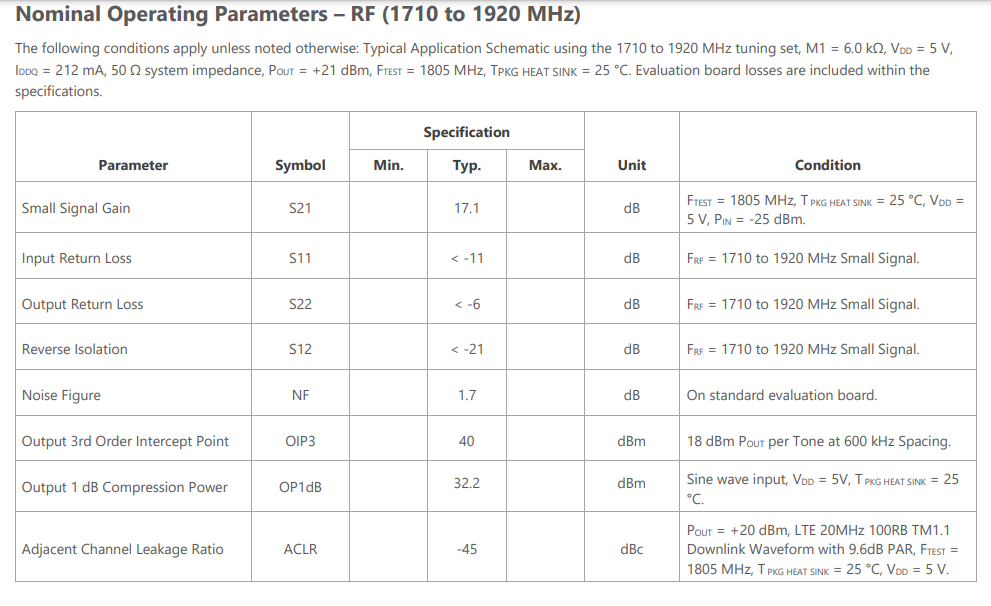
\includegraphics{DatasheetImages/poweramptable.png}}
  \caption{Power Amplifier Table}
  \label{img:poweramptable}
\end{figure}
At this point after the VCO and phase shifter, we want the RF signal to propogate through the air. However, according to the
radar range equation the power of the signal when attenuating through the air attenuates at a power of four which is a lot.
Therefore, we need to make sure our signal is powerful enough to go pretty far. So, we use an RF power amplifier to amplify the
signal. We chose a part from GuerillaRF which can be found \href{https://www.mouser.com/ProductDetail/Guerrilla-RF/GRF5112?qs=ulEaXIWI0c%252Bti188Qa1Now%3D%3D}{here}.
Looking at the table in Figure \ref{img:poweramptable}, we can see some key metrics when looking at power amplifiers. First,
of course we want to make sure it has a bandwidth that supports our chosen frequency of 1.8 GHz. Second, we want to look at the
small-signal gain and Output 1 dB Compression Point or OP1dB. The small-signal gain is the ideal gain that can be reached with a 
low power signal, and is listed as 17.1 dB. The OP1dB is a metric we did not know about and were thankful to find it. With most amplifiers,
gain operates linearly meaning whatever power your input signal is you just add the gain of the amplifier and this will be the resulting power of the signal.
However, at a certain point the amplifier saturates and does not operate linearly anymore, and will essentially cap-off its gain at
the OP1dB limit. For example, with the OP1dB being 32.2 dB, if I input a signal that was 30 dB I would expect a resulting signal of
47.1 dB but this would not be the case. The amplifier ceases to operate linearly after the 32.2 dB mark, and will both distort the signal
and output something weaker than expected. A lot of amplifiers will boast a high gain but have a low OP1dB, so this is definitely something to check for.

\section{Low Noise Amplifier}
\begin{figure}[H]
  \centering
  \scalebox{.7}{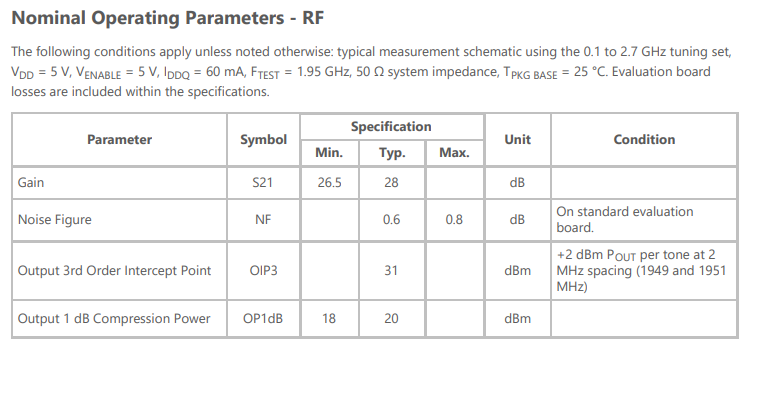
\includegraphics{DatasheetImages/lnatable.png}}
  \caption{Low-Noise Amplifier Table}
  \label{img:lnatable}
\end{figure}

This is the first part that will be placed in the receiver RF chain. According to the Friis equation in Chapter \ref{Radar Theory},
the first stage in the receiver RF chain matters a lot for the noise figure of your system. Therefore, we wanted to find a part
with a low noise figure and high gain, as this will impact our SNR the most. Low noise amplifiers are made for this exact purpose,
where they amplify a small signal with very low noise. The part we chose was \href{https://www.mouser.com/ProductDetail/Guerrilla-RF/GRF2133W?qs=ulEaXIWI0c%2FXgAPwqRmr2A%3D%3D}{this},
which is made by GuerillaRF. By examining the table in Figure \ref{img:lnatable}, we can see that it has a gain of 28 dB,
and a noise figure of .6 dB. We also can look at the OP1dB which has a figure of 20 dB. Since the LNA will be amplifying a signal
straight from an antenna, the signal will be super weak and there is a low likelihood it will reach the OP1dB.

\section{Mixer/LO Amp}
\begin{figure}[H]
  \centering
  \scalebox{.7}{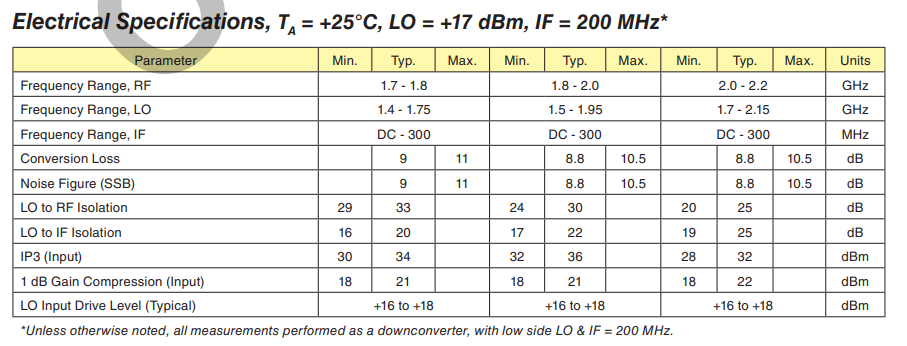
\includegraphics{DatasheetImages/mixertable.png}}
  \caption{Mixer Table}
  \label{img:mixertable}
\end{figure}
\begin{figure}[H]
  \centering
  \scalebox{.7}{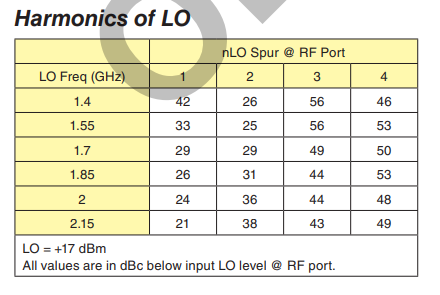
\includegraphics{DatasheetImages/mixerharmonics.png}}
  \caption{Mixer Harmonics Table}
  \label{img:mixerharmonics}
\end{figure}

Now that our received signal is amplified we must down-convert it in order to sample and process it. The process for doing
this is called heterodyning or mixing, and the theory behind this can be found in detail in Chapter \ref{Radar Theory}. 
A mixer has three ports, the local oscillator, RF signal, and output. The local oscillator and RF signal are multiplied
to produce the sum and difference of the LO and RF signals on the output port. We are mainly interested in the difference,
also called the Intermediate Frequency (IF) since it is a low frequency and can be sampled easily.
In our case, we take a copy of the VCO as the local oscillator and then mix this with the amplified return signal 
to produce our intermediate frequency. To achieve this, we used a discontinued mixer from Analog Devices which
can be found \href{https://www.arrow.com/en/products/hmc400ms8etr/analog-devices}{here}. 
Looking at the mixer's specifications table in Figure \ref{img:mixertable}, we can 
see some new properties. The conversion loss is the output IF power delivered minus the available RF input signal power. The
LO to RF Isolation is how much of the local oscillator signal leaks into the RF port, and the LO to IF Isolation is how much
the local oscillator signal leaks into the output port. This is a passive component, meaning it does not require power and
solely operates off the power of the LO and RF signals. Therefore we see in the table that the LO Input must be 16-18 dBm to drive
the mixer. Essentially the local oscillator powers the mixer, and its harmonics will therefore be prominent in the IF port due to
leakage. We can see in Figure \ref{img:mixerharmonics} that at 1.85 GHz the manufacturer tells us the strength of LO harmonics 
up to the fourth order. At the top it says spur which means spurious (unwanted) outputs due to the nonlinearity of the mixer.
Essentially this table tells us that there will be unwanted spectral components in the output, which is something we did not
pay enough attention to and will discuss in Chapter \ref{Issues}.
\begin{figure}[H]
  \centering
  \scalebox{.7}{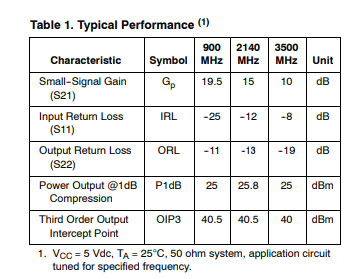
\includegraphics{DatasheetImages/loamptable.png}}
  \caption{LO Amp Table}
  \label{img:loamptable}
\end{figure}

As we said before, the mixer is a passive component which is driven by the LO which needs a power level of 16-18 dBm.
After splitting our VCO's output four ways, we have about a ~2 dBm signal that we must amplify. So, we chose an RF broadband
amplifier from NXP which can be found \href{https://www.digikey.com/en/products/detail/nxp-usa-inc/MMG3014NT1/1971761}{here}. As
we can see in Figure \ref{img:loamptable}, the amp has a gain of around 15 dB for our frequency and an OP1dB of 25.8 dB which is
a lot of headroom.

\section{IF Amplifiers and Filters}
Now, our return signal has been downconverted, but the power of that signal is very weak. As well as this, there are unwanted
spectral components in that signal that are bi-products of the mixer that we need to get rid of. This means we need amplifiers and
filters to make our signal ready to be sampled and processed in the microcontroller. First we used a super simple op-amp
that served as a voltage follower which can be found \href{https://www.digikey.com/en/products/detail/microchip-technology/MCP6001UT-I-OT/562450}{here}.
This was used to create a virtual ground for our biasing. Then we use a dual channel op-amp from TI for our variable gain
amplifier which can be found \href{https://www.mouser.com/ProductDetail/Texas-Instruments/LM2904DR?qs=5BZzbFV4k2vkQqOl3Q8qPg%3D%3D}{here}.

\begin{figure}[H]
  \centering
  \scalebox{.7}{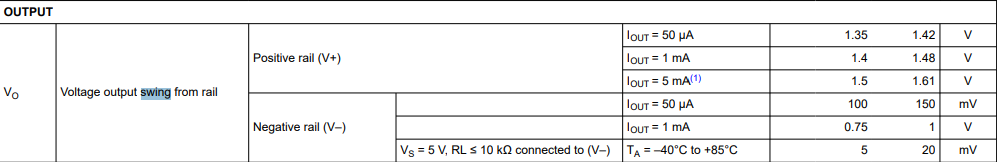
\includegraphics{DatasheetImages/outputswing.png}}
  \caption{Output Swing Characteristics}
  \label{img:outputswing}
\end{figure}

Honestly, when selecting parts we figured all operational amplifiers just acted the same way. However, after printing and manufacturing
we ran into problems which will be discussed in Chapter \ref{Issues} that could have been remedied if we paid more attention to
the Op-Amps we were using. The main problem is that these operational amplifiers are not "Rail-to-Rail".
While rail-to-rail amplifiers guarantee that they do not saturate until the positive and negative voltages you've supplied it,
other amplifiers have what is called voltage swing. As we can see in Figure \ref{img:outputswing}, the range of voltage
that the operational amplifier can achieve is not its rails, but specifies how much lower than its rail it will be. This is 
something to look out for when selecting an Op-Amp.

\begin{figure}[H]
  \centering
  \scalebox{.7}{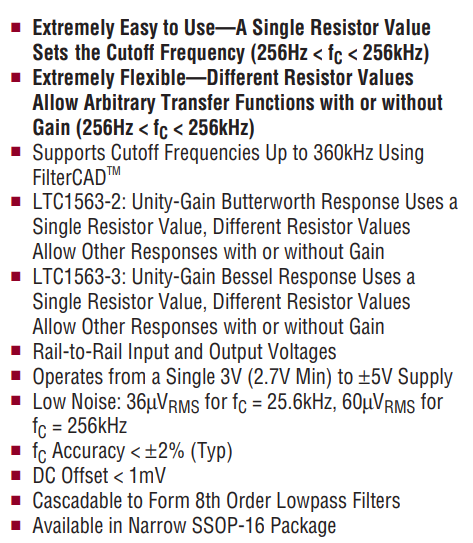
\includegraphics{DatasheetImages/filterspecs.png}}
  \caption{Filter Features}
  \label{img:filterspecs}
\end{figure}

After amplifying the signal, we wanted to filter out unwanted spectral components by using a strong filter. Instead of designing
this ourselves, we decided to use a 4th Order LPF which can be found \href{https://www.digikey.com/en/products/detail/analog-devices-inc/LTC1563-2IGN-PBF/962958}{here}.
By looking at Figure \ref{img:filterspecs}, we can see that this is an integrated circuit with a flexible cutoff frequency.
It also says that it is a rail-to-rail input and output circuit, which is an important feature to note as discussed with the amplifiers.
A fourth order filter just means that this filter has four filters with the same cutoff frequency cascaded upon each other, which
yields a steeper frequency response and attenuates are unwanted signals further.
\chapter{PCB
\index{Chapter!PCB}
\index{PCB}
\label{PCB}}
\chapter{Digital Processing
\index{Chapter!Digital Processing}
\index{Digital Processing}
\label{Digital Processing}}
\chapter{Networking
\index{Chapter!Networking}
\index{Networking}
\label{Networking}}


\chapter{Results
\index{Chapter!Results}
\index{Results}
\label{Results}}
\chapter{Issues
\index{Chapter!Issues}
\index{Issues}
\label{Issues}}

%\bibliography{bibfile}
%\bibliographystyle{unsrt}
%\bibliographystyle{IEEEtran}

%% Initial version by Darian Muresan, Ph.D.
% Edit and adjust as needed.

\documentclass[12pt]{cornell}

% add index support
\makeindex

% graphing programs
\usepackage{color}
\usepackage{psfrag}
\usepackage{verbatim}
\usepackage{fancyhdr}
\usepackage{minted}
%\usepackage{titlesec}
\usepackage{fancyvrb} 
% hyperlink programs
\usepackage[luatex, 
breaklinks=true, 
colorlinks=true,
citecolor=blue,
linkcolor=blue,
menucolor=black,
pagecolor=black,
urlcolor=blue
]{hyperref} % links in pdf
%\usepackage[colorlinks]{hyperref} % links in dvi
\usepackage{listings}
\usepackage{amsfonts} 
\usepackage{amssymb} 
%\usepackage{tabto}

\usepackage{tabularx,colortbl}
\usepackage[chapter]{algorithm} 
\usepackage{algorithmic} 
\usepackage{blindtext}
\usepackage{imakeidx}

% for electronics:
\usepackage[american]{circuitikz}

\definecolor{DarkGreen}{rgb}{0,0.6,0}
\definecolor{mygreen}{rgb}{0,0.6,0}
\definecolor{mygray}{rgb}{0.5,0.5,0.5}
\definecolor{mymauve}{rgb}{0.58,0,0.82}

\usepackage{tocloft}
\usepackage{amsmath}
\usepackage{tcolorbox}
\usepackage{enumitem}
\usepackage{longtable}
%\usepackage{textcomp}
\usepackage{txfonts}

%part for \part titles
%chap for \chapter titles
%sec for \section titles
%subsec for \subsection titles
%subsubsec for \subsubsection titles
%para for \paragraph titles
%subpara for \subparagraph titles
%fig for figure \caption titles
%subfig for subfigure \caption titles
%tab for table \caption titles
%subtab for subtable \caption titles

% update chapter number spacing
\setlength{\cftchapnumwidth}{2em}
\setlength{\cftsecnumwidth}{2.5em}
\setlength{\cftsubsecnumwidth}{3.5em}
\setlength{\cftsubsubsecnumwidth}{4.5em}

\addtolength{\cftsecindent}{0.5em}
\addtolength{\cftsubsecindent}{0.5em}
\addtolength{\cftsubsubsecindent}{0.5em}

%\titlespacing*{\chapter}{0pt}{-50pt}{20pt}
%\titleformat{\chapter}[display]{\normalfont\huge\bfseries}{\chaptertitlename\ 
%\thechapter}{20pt}{\Huge}
%\pagestyle{fancy}
%\pagestyle{cornell}
%
%\rhead{F054-021-0172}
%\chead{Nonlinear Enhancement of Visual Target Detection (AF05-T021)}
%\lhead{GSTI}
%\lfoot{\scriptsize Use or disclosure of data on this page is subject
%to the restriction on the title page of this proposal.}
%\cfoot{}
%\rfoot{\thepage}

\newfont{\Bp}{msbm10}
\newfont{\BpBig}{msbm10 scaled\magstep2}
\newfont{\Sc}{eusm10}
\newfont{\ScBig}{eusm10 scaled\magstep3}
\newfont{\Fr}{eufm10}
\newfont{\FrBig}{eufm10 scaled\magstep1}

% some commands:
\newcommand{\dxi}{{\tt m\_xDeltaInput}}
\newcommand{\dyi}{{\tt m\_yDeltaInput}}
\newcommand{\dci}{{\tt m\_cDeltaInput}}
\newcommand{\dxo}{{\tt m\_xDeltaOutput}}
\newcommand{\dyo}{{\tt m\_yDeltaOutput}}
\newcommand{\dco}{{\tt m\_cDeltaOutput}}
\newcommand{\ttf}[1]{{\tt #1}}
\newcommand{\tbl}[2]{{\begin{tabular}{c} #1 \\ #2 \end{tabular}}}

\newcommand{\urltwo}[2]{\mbox{\href{#1}{\tt #2}}}
\newcommand{\qnorm}[1]{\|#1\|_{\bQ}}
\newcommand{\qdot}[2]{\lrb #1, #2 \rrb_{\bQ}}
\newcommand{\kdot}[2]{\lrb #1, #2 \rrb_{\bf k}}
\newcommand{\tdot}[2]{\lrb #1, #2 \rrb}
\newcommand{\mydiff}[2]{\lrb #1 - #2 \rrb}
\newcommand{\lena}{\textit{lena}}
\newcommand{\barb}{\textit{barbara}}
\newcommand{\boat}{\textit{boat}}
\newcommand{\leaves}{\textit{leaves}}
\newcommand{\rings}{\textit{rings}}
\newcommand{\treg}{\textit{train region}}
\newcommand{\dreg}{\textit{denoise region}}
\newcommand{\oreg}{\textit{overlap region}}
\newcommand{\sil}{\sigma_l^2}
\newcommand{\sn}{\sigma^2}
\newcommand{\bn}{{\mbox{\bf \FrBig N}}}
\newcommand{\n}{\mbox{\Fr N}}
%\newcommand{\bn}{\bf N}
%\newcommand{\n}{N}
\newcommand{\bY}{\textbf{Y}}
\newcommand{\bX}{\textbf{X}}
\newcommand{\bb}{\textbf{b}}
\newcommand{\bu}{\textbf{u}}
\newcommand{\bv}{\textbf{v}}
\newcommand{\by}{\textbf{y}}
\newcommand{\bx}{\textbf{x}}
\newcommand{\be}{\textbf{e}}
\newcommand{\bz}{\textbf{z}}
\newcommand{\bs}{\textbf{s}}
\newcommand{\bw}{\textbf{w}}
\newcommand{\bQ}{\textbf{Q}}
\newcommand{\bphi}{\textbf{$\phi$}}
\newcommand{\lsb}{\left[}
\newcommand{\rsb}{\right]}
\newcommand{\lrb}{\left(}
\newcommand{\rrb}{\right)}
\newcommand{\lcb}{\left\{}
\newcommand{\rcb}{\right\}}
\newcommand{\R}{\mbox{\BpBig R}}
\newcommand{\F}{{\cal F}}
\newcommand{\Fk}{\mbox{\Sc F}}
\newcommand{\bQF}{\textbf{Q}_{\mbox{\Sc F}}}
\newcommand{\N}{{\cal N}}
\newcommand{\xlz}{X_l(z)}
\newcommand{\xhz}{X_h(z)}
\newcommand{\xz}{X(z)}
\newcommand{\pr}{ perfect reconstruction }
\newcommand{\smb}{Smith-Barnwell }
\newcommand{\xw}{X(e^{j\omega})}
\newcommand{\xmw}{X(-e^{j\omega})}
\newcommand{\dw}{D(e^{j\omega})}
\newcommand{\dmw}{D(-e^{j\omega})}
\newcommand{\ew}{E(e^{j\omega})}
\newcommand{\emw}{E(-e^{j\omega})}
\newcommand{\fw}{F_0(e^{j\omega})}
\newcommand{\fmw}{F_0(-e^{j\omega})}
\newcommand{\hoz}{H_1(z)}
\newcommand{\hzz}{H_0(z)}
\newcommand{\goz}{G_1(z)}
\newcommand{\gzz}{G_0(z)}
\newcommand{\hzw}{H_{0}(e^{j\omega})}
\newcommand{\hzmw}{H_{0}(-e^{j\omega})}
\newcommand{\hzcw}{H_{0}(e^{-j\omega})}
\newcommand{\how}{H_1(e^{j\omega})}
\newcommand{\homw}{H_1(-e^{j\omega})}
\newcommand{\gzw}{G_0(e^{j\omega})}
\newcommand{\gzmw}{G_0(-e^{j\omega})}
\newcommand{\gow}{G_1(e^{j\omega})}
\newcommand{\gomw}{G_1(-e^{j\omega})}
\newcommand{\wl}{e^{-jwL}}
\newcommand{\aqua}{\textit{AQua with OR }}
\newtheorem{theorem}{Theorem}
\newtheorem{lemma}{Lemma}
\newtheorem{corollary}{Corollary}
\newtheorem{claim}{Claim}
\newtheorem{definition}{Definition}
\newenvironment{proof}{\noindent{\em Proof.}}{\ \hfill Q.E.D.}
%\newtheorem{moduleCount}{L}
\newcommand*{\labelfile}[1]{%
  \label{file:#1}%
}

\lstset{ %
  backgroundcolor=\color{white},   % choose the background color; you must add \usepackage{color} or \usepackage{xcolor}
  basicstyle=\footnotesize,        % the size of the fonts that are used for the code
  breakatwhitespace=false,         % sets if automatic breaks should only happen at whitespace
  breaklines=true,                 % sets automatic line breaking
  captionpos=b,                    % sets the caption-position to bottom
  commentstyle=\color{DarkGreen},    % comment style
  deletekeywords={...},            % if you want to delete keywords from the given language
  escapeinside={\%*}{*)},          % if you want to add LaTeX within your code
  extendedchars=true,              % lets you use non-ASCII characters; for 8-bits encodings only, does not work with UTF-8
  %frame=single,                   % adds a frame around the code
  keepspaces=true,                 % keeps spaces in text, useful for keeping indentation of code (possibly needs columns=flexible)
  keywordstyle=\color{blue},       % keyword style
  language=C++,                    % the language of the code
  morekeywords={*,...},            % if you want to add more keywords to the set
  numbers=left,                    % where to put the line-numbers; possible values are (none, left, right)
  numbersep=5pt,                   % how far the line-numbers are from the code
  numberstyle=\tiny\color{mygray}, % the style that is used for the line-numbers
  rulecolor=\color{black},         % if not set, the frame-color may be changed on line-breaks within not-black text (e.g. comments (green here))
  showspaces=false,                % show spaces everywhere adding particular underscores; it overrides 'showstringspaces'
  showstringspaces=false,          % underline spaces within strings only
  showtabs=false,                  % show tabs within strings adding particular underscores
  stepnumber=1,                    % the step between two line-numbers. If it's 1, each line will be numbered
  stringstyle=\color{mymauve}     % string literal style
  %tabsize=2,                      % sets default tabsize to 2 spaces
  %caption=\lstname                % show the filename of files included with \lstinputlisting; also try caption instead of title
}

% Uncomment draftcopy to get the word DRAFT boldly across the first page
%   By the way, xdvi won't show it but it will come out when you print
%\usepackage[light,all]{draftcopy}		% DRAFT on first page
%\draftcopySetGrey{.97}
%\draftcopyName{Confidential}{150}
%\draftcopFirstPage{1}

% Uncomment drafthead to get the date and DRAFT in the header of pages
% that are normallly numbered on the top, pages 2-n of each chapter for example
% This doesn't work with centered page numbers: \pagestyle{cornellc}
%\usepackage{drafthead}

% Including selective chapters:
% use this to selectively process chapters, etc.  Put a % in front of
% the sections that you don't want done this time.  Includes are
% used instead of \input so that LaTeX will keep track of chapters and
% pages without processing everything.  Don't let any spaces creep in
% around the words or it will not work!


\includeonly{
prologue,
manIntroduction,
manProjectDescription,
manResources,
manRadarTheory,
manPartSelection,
manPCB,
manDigitalProcessing,
manNetworking,
manResults,
manIssues
}

\makeindex

\begin{document}

\pagenumbering{roman}
\singlespacing
\include{prologue}

\setcounter{page}{1}        % set page counter
\pagenumbering{arabic}      % set page number style
\pagestyle{fancy}         % top right page numbers
%\pagestyle{cornell}
%\pagestyle{cornellc}       % centered page numbers, disables drafthead

\renewcommand{\chaptermark}[1]{\markboth{#1}{}}
\renewcommand{\sectionmark}[1]{\markright{#1}{}}

\fancyhead{} % clear all fields

\lhead{Chapter \thechapter}
%\lhead{\thechapter}
\chead{\leftmark}
\rhead{\thepage}


\lfoot{Chapter \thechapter}
\cfoot{\copyright Stevens -- \today \mbox{} -- FPGA Radio Receiver/Transmitter}
\rfoot{\thepage}

\renewcommand{\headrulewidth}{0.4pt}
\renewcommand{\footrulewidth}{0.4pt}

%\rhead{F054-021-0172}
%\chead{Nonlinear Enhancement of Visual Target Detection (AF05-T021)}
%\lhead{GSTI}
%\lfoot{\scriptsize Use or disclosure of data on this page is subject
%to the restriction on the title page of this proposal.}
%\cfoot{}
%\rfoot{\thepage}


\singlespacing
\include{manIntroduction}
\include{manProjectDescription}
\include{manResources}
\include{manRadarTheory}
\include{manPartSelection}
\include{manPCB}
\include{manDigitalProcessing}
\include{manNetworking}
\include{manResults}
\include{manIssues}

%\bibliography{bibfile}
%\bibliographystyle{unsrt}
%\bibliographystyle{IEEEtran}

%\input{manual.ind}
\printindex
\end{document}

\printindex
\end{document}

\printindex
\end{document}

\printindex
\end{document}
